%!TEX TS-program = lualatex
%!TEX encoding = UTF-8 Unicode
\documentclass[leqno, openany]{memoir}
\setulmarginsandblock{3.5cm}{3.5cm}{*}
\setlrmarginsandblock{3cm}{3.5cm}{*}
\checkandfixthelayout

\usepackage{amsmath}
\usepackage{amssymb}
\usepackage{amsthm}
\usepackage{bm}
\usepackage{stmaryrd}
\usepackage{accents}
\usepackage{mathtools}
\usepackage{tikz}
\usetikzlibrary{calc}
\usetikzlibrary{automata,positioning}
\usepackage{tikz-cd}
\usepackage{forest}
\usepackage{braket} 
\usepackage{listings}
\usepackage{mdframed}
\usepackage{verbatim}
\usepackage{graphicx}
\graphicspath{ {./} }
\usepackage{physics}
%\usepackage{/home/patrickl/homework/macaulay2}

% font
\usepackage{fontspec}
\usepackage{unicode-math}
\setmainfont[Ligatures={Common}, Numbers={OldStyle}]{Libertinus Serif}
\setsansfont[Ligatures={Common}, Numbers={OldStyle}]{Libertinus Sans}
\setmonofont{Inconsolata}
\setmathfont{Libertinus Math}

%CS packages
\usepackage{algorithmicx}
\usepackage{algpseudocode}
\usepackage{algorithm}

% typeset and bib
\usepackage[english]{babel} 
\usepackage[utf8]{inputenc} 
\usepackage[backend=biber, style=alphabetic]{biblatex}
\usepackage[bookmarks, colorlinks, breaklinks]{hyperref} 
\hypersetup{linkcolor=black,citecolor=black,filecolor=black,urlcolor=black}
\usepackage{microtype}

% other formatting packages
\usepackage{float}
\usepackage{booktabs}
\usepackage{enumitem}
\usepackage{csquotes}
\usepackage{titlesec}
\usepackage{titling}
\usepackage{fancyhdr}
\usepackage{lastpage}
\usepackage{parskip}

\usepackage{lipsum}

% delimiters
\DeclarePairedDelimiter{\gen}{\langle}{\rangle}
\DeclarePairedDelimiter{\floor}{\lfloor}{\rfloor}
%\DeclarePairedDelimiter{\abs}{\lvert}{\rvert}
\DeclarePairedDelimiter{\ceil}{\lceil}{\rceil}
%\DeclarePairedDelimiter{\norm}{\lVert}{\rVert}


\newtheorem{thm}{Theorem}[chapter]
\newtheorem{cor}[thm]{Corollary}
\newtheorem{prop}[thm]{Proposition}
\newtheorem{lem}[thm]{Lemma}
\newtheorem{conj}[thm]{Conjecture}
\newtheorem{quest}[thm]{Question}

\theoremstyle{definition}
\newtheorem{defn}[thm]{Definition}
\newtheorem{defns}[thm]{Definitions}
\newtheorem{con}[thm]{Construction}
\newtheorem{exm}[thm]{Example}
\newtheorem{exms}[thm]{Examples}
\newtheorem{notn}[thm]{Notation}
\newtheorem{notns}[thm]{Notations}
\newtheorem{addm}[thm]{Addendum}
\newtheorem{exer}[thm]{Exercise}

\theoremstyle{remark}
\newtheorem{rmk}[thm]{Remark}
\newtheorem{rmks}[thm]{Remarks}
\newtheorem{warn}[thm]{Warning}
\newtheorem{sch}[thm]{Scholium}


% unnumbered theorems
\theoremstyle{plain}
\newtheorem*{thm*}{Theorem}
\newtheorem*{prop*}{Proposition}
\newtheorem*{lem*}{Lemma}
\newtheorem*{cor*}{Corollary}
\newtheorem*{conj*}{Conjecture}

% unnumbered definitions
\theoremstyle{definition}
\newtheorem*{defn*}{Definition}
\newtheorem*{exer*}{Exercise}
\newtheorem*{defns*}{Definitions}
\newtheorem*{con*}{Construction}
\newtheorem*{exm*}{Example}
\newtheorem*{exms*}{Examples}
\newtheorem*{notn*}{Notation}
\newtheorem*{notns*}{Notations}
\newtheorem*{addm*}{Addendum}


\theoremstyle{remark}
\newtheorem*{rmk*}{Remark}

% shortcuts
\newcommand{\Ima}{\mathrm{Im}}
\newcommand{\A}{\mathbb{A}}
\newcommand{\R}{\mathbb{R}}
\renewcommand{\C}{\mathbb{C}}
\newcommand{\Z}{\mathbb{Z}}
\newcommand{\Q}{\mathbb{Q}}
\renewcommand{\k}{\Bbbk}
\renewcommand{\P}{\mathbb{P}}
\newcommand{\M}{\overline{M}}
\newcommand{\g}{\mathfrak{g}}
\newcommand{\h}{\mathfrak{h}}
\newcommand{\n}{\mathfrak{n}}
\renewcommand{\b}{\mathfrak{b}}
\newcommand{\ep}{\varepsilon}
\newcommand*{\dt}[1]{%
   \accentset{\mbox{\Huge\bfseries .}}{#1}}
\renewcommand{\abstractname}{Official Description}
\newcommand{\mc}[1]{\mathcal{#1}}
\newcommand{\T}{\mathbb{T}}
\newcommand{\mf}[1]{\mathfrak{#1}}
\newcommand{\mr}[1]{\mathrm{#1}}
\newcommand{\wt}[1]{\widetilde{#1}}

\DeclareMathOperator{\Der}{Der}
\DeclareMathOperator{\Hom}{Hom}
\DeclareMathOperator{\End}{End}
\DeclareMathOperator{\ad}{ad}
\DeclareMathOperator{\Aut}{Aut}
\DeclareMathOperator{\Rad}{Rad}
\DeclareMathOperator{\supp}{supp}
\DeclareMathOperator{\sgn}{sgn}
\DeclareMathOperator{\Bl}{Bl} %blowup


\titleformat{\section}
    {\Large\sffamily\scshape\bfseries}{\thesection}{1em}{}
\titleformat{\subsection}[runin]
    {\large\sffamily\bfseries}{\thesubsection}{1em}{}
\titleformat{\subsubsection}[runin]{\sffamily\itshape}{\thesubsubsection}{1em}{}

\title{COURSE TITLE}
\author{Lectures by INSTRUCTOR, Notes by Patrick Lei}
\date{SEMESTER}

\newcommand*{\titleSW}
    {\begingroup% Story of Writing
    \raggedleft
    \vspace*{\baselineskip}
    {\Huge\itshape Symplectic Topology \\ Math 705}\\[\baselineskip]
    {\large\itshape Notes by Patrick Lei,
                    Spring 2020}\\[0.2\textheight]
                    {\Large Lectures by R. \.Inan\c{c} Baykur}\par
    \vfill
    {\Large \sffamily University of Massachusetts Amherst}
    \vspace*{\baselineskip}
\endgroup}
\pagestyle{simple}

\chapterstyle{ell}


%\renewcommand{\cftchapterpagefont}{}
\renewcommand\cftchapterfont{\sffamily}
\renewcommand\cftsectionfont{\sffamily\scshape}
\renewcommand*{\cftchapterleader}{}
\renewcommand*{\cftsectionleader}{}
\renewcommand*{\cftsubsectionleader}{}
\renewcommand*{\cftchapterformatpnum}[1]{~\textbullet~#1}
\renewcommand*{\cftsectionformatpnum}[1]{~\textbullet~#1}
\renewcommand*{\cftsubsectionformatpnum}[1]{~\textbullet~#1}
\renewcommand{\cftchapterafterpnum}{\cftparfillskip}
\renewcommand{\cftsectionafterpnum}{\cftparfillskip}
\renewcommand{\cftsubsectionafterpnum}{\cftparfillskip}
\setrmarg{3.55em plus 1fil}
\setsecnumdepth{subsection}
\maxsecnumdepth{subsection}
\settocdepth{subsection}

\begin{document}
    
\begin{titlingpage}
\titleSW
\end{titlingpage}

\thispagestyle{empty}
\section*{Disclaimer}%
\label{sec:disclaimer}

These notes were taken during lecture using the \texttt{vimtex} package of the editor \texttt{neovim}. 
Any errors are mine and not the instructor's. 
In addition, my notes are picture-free (but will include commutative diagrams) and are a mix of my mathematical style 
(omit lengthy computations, use category theory) and that of the instructor.
If you find any errors, please contact me at \texttt{plei@umass.edu}.
\newpage



\tableofcontents

\chapter{January 21}%
\label{cha:january_21}

\section{Course Description}%
\label{sec:course_description}

This is an introductory course on symplectic topology, along with its connections to differential, complex algebraic, and contact geometry and topology.

\section{Organization}%
\label{sec:organization}

\.Inan\c{c} passed around a syllabus. Prerequisites for this course are smooth manifolds, some algebraic topology (cohomology), and complex analysis. Because this is a second year graduate course, we are expected to read any missing background on our own. Grading will be based on homework and a final presentation. We will cover the first four topics on the syllabus and do some of the last four. Finally, \.Inan\c{c} may add more geometry to the course.

\subsection{Notational conventions}%
\label{sub:notational_conventions}

We will denote finite dimensional real vector spaces over $\R$ by $V$ and smooth manifolds by $M$.

\section{Basic Notions}%
\label{sec:basic_notions}

\begin{defn}
    A \textit{symplectic form} (or a \textit{symplectic} structure) on a vector space $V$ is a nondegenerate alternating bilinear form $V \otimes V \to \R$.
\end{defn}

\begin{defn}
    A \textit{symplectic form} (or symplectic structure) on a smooth manifold $M$ is a differential form $\omega \in \Omega^2 M$ which is closed and everywhere nondegenerate.
\end{defn}

\begin{rmk}
A fundamental question to ask is when a manifold admits a symplectic structure. We will see that symplectic structures exist only on even-dimensional manifolds. Saying more is an extremely difficult problem, although we can say that symplectic manifolds admit an almost complex structure and are orientable. Uniqueness up to both symplectomorphism and deformation is also very difficult.
\end{rmk}

\begin{exm}
    Let $V = \R^{2n}$ with coordinates $x_1, \ldots, x_n, y_1, \ldots, y_n$. Then we can define a form
    \[ \omega_0(u,v) = \sum_{i=0}^n (x_i y_i' - x_i'y_i) = -u^T J_0 v, \]
    where 
    \[J_0 = \begin{pmatrix}
        0 & -I_n \\
        I_n & 0
    \end{pmatrix}.\]
    Checking that $\omega_0$ is a nondegenerate alternating bilinear form is easy. Later we will see that this is the only symplectic vector space.
\end{exm}

\begin{exm}
    Consider $M = \R^{2n}$ with coordinates $x_1, y_1, \ldots, x_n, y_n$. Now consider the form
    \[ \omega_0 = \sum_{i=1}^n dx_i \wedge dy_i.\] 
    Checking that this form is closed and nondegenerate is easy. We can also define the form on $\C^n$, where the form becomes 
    \[ \frac{i}{2} \sum_{i=j}^n dz_j \wedge d \overline{z_j}.\]
\end{exm}

Note that the requirement that symplectic forms are closed is a subtle condition. If we multiply by a general function, the resulting form will not be closed. Recall that smooth manifolds are locally Euclidean. We can require our transitions to lie in the symplectic group, and later we will show that this definition of a symplectic manifold is equivalent to the one we gave today.

For a general manifold $M$, we want to associate linear spaces to it. 

\begin{defn}
    A vector bundle $E$ over $M$ is a \textit{symplectic vector bundle} if there exists a smooth section $\omega$ of $E^* \wedge E^*$ such that $(E_x, \omega_x)$ is a symplectic vector space for all $x \in M$.
\end{defn}

\begin{exm}
    For a symplectic manifold $M$, the tangent bundle $TM$ is a symplectic vector bundle.
\end{exm}

\begin{rmk}
    Observe that if the tangent bundle is symplectic, then the manifold is not necessarily symplectic.
\end{rmk}

\section{Symplectic Linear Algebra}%
\label{sec:symplectic_linear_algebra}

\begin{defn}
    For $(V_i, \omega_i)$ symplectic vector spaces, a \textit{linear symplectomorphism} $\phi: (V_1, \omega_1) \to (V_2, \omega_2)$ is an isomorphism of vector spaces such that $\phi^* \omega_2 = \omega_1$. They $(V_1, \omega_1)$ and $(V_2, \omega_2)$ are \textit{symplectomorphic}.
\end{defn}

The usual definition of orthogonal complements carries over and will be denoted $W^{\omega}$ for a subspace $W \subset V$.

\begin{lem}
    Let $(V, \omega)$ be a symplectic vector space.
    \begin{enumerate}
        \item $v \mapsto \omega(v,-)$ is an isomorphism $V \to V^*$.
        \item $\dim W + \dim W^{\omega} = \dim V$.
        \item ${ (W^{\omega}) }^{\omega} = W$.
        \item The following are equivalent:
            \begin{enumerate}
                \item $W$ is a symplectic subspace of $V$;
                \item $W^{\omega}$ is symplectic;
                \item $W \cap W^{\omega} = \{0\}$;
                \item $W \oplus W^{\omega} = V$.
            \end{enumerate}
    \end{enumerate}
\end{lem}

\begin{proof}
    \begin{enumerate}
        \item This part is equivalent to nondegeneracy.
        \item Use a rank-nullity argument to note that $W^{\omega}$ maps to the annihlator of $W$ under the isomorphism $V \to V^*$.
        \item Clearly $W \subset { (W^{\omega}) }^{\omega}$. Then use the dimension result.
        \item Clearly a) implies c) and c) and d) are equivalent. Finally, it is easy to see that d) implies a). Finally equivalence of b) to the rest is easy.
    \end{enumerate}
\end{proof}

\begin{thm}[Symplectic Basis]
    For any symplectic vector space $(V, \omega)$, there exists a basis $u_1, \ldots, u_n, v_1, \ldots, v_n$ such that
    \[ \omega(u_i,u_j) = 0, \omega(v_i, v_j) = 0, \omega(u_i, v_j) = \delta_{ij},\]
    called a \textit{symplectic basis for $(V, \omega)$}.
\end{thm}

\chapter{January 23}%
\label{cha:january_23}

\section{More Basic Linear Algebra}%
\label{sec:more_basic_linear_algebra}

Last time we stated the following:
\begin{thm*}
    For any symplectic vector space $(V, \omega)$, there exists a basis $u_1, \ldots, u_n, v_1, \ldots, v_n$ such that $\omega(u_i, v_i) = 1$ and any other pairing is zero.
\end{thm*}

\begin{proof}
    We will induct on the dimension of the vector space. For $n = 1$, take any nonzero $u$. Then by nondegeneracy, we can find a desired $v$. Then we simply use Lemma 1.4.2, note that $u_1, v_1$ span a symplectic subspace $W$ of $V$, and apply the inductive hypothesis to $W^{\omega}$. Because $u_1, v_1$ are orthogonal to the symplectic basis for $W^{\omega}$, we are done.
\end{proof}

\begin{cor}
    Any symplectic vector space is symplectomorphic to $(\R^{2n}, \omega_0)$.
\end{cor}

\begin{proof}
    Observe that 
    \[ \omega = \sum_{i=1}^n u_i^* \wedge v_i^*. \]
    Define our morphism in the obvious way:
    \[ (x_1, \ldots, x_n, y_1, \ldots, y_n) \mapsto \sum x_i u_i + y_i v_i.\]
    Then it is easy to check that
    \[ \phi^* \omega (x,x') = \omega(\phi x, \phi x') = \left( \sum u_i^* \wedge v_i^* \right) \left( \sum x_i u_i + y_i v_i, \sum x_i' u_i + y_i' v_i \right) = \sum x_i y_i' - x_i' y_i = \omega_0(x,x').\]
\end{proof}

\begin{cor}
    A skew-symmetric $\omega$ on $V$ is symplectic iff $\omega^n \neq 0$.
\end{cor}

\begin{proof}
    If $\omega$ is symplectic, then there exists a symplectic basis $\{ u_i, v_i \}$, and $\omega^n(u_1, v_1, \ldots, u_n, v_n) \neq 0$. In the other direction, if $\omega$ is degenerate, there exists $u \in 0$ such that $\omega(u,v) = 0$ for all $v \in V$. Then we can complete $u$ to a basis by $u_2, \ldots, u_{2n}$, and here $\omega^n(u, u_2, \ldots, u_{2n}) = 0$, so $\omega^n = 0$.
\end{proof}

\section{Compatible Complex Structures and Inner Products}%
\label{sec:compatible_complex_structures_and_inner_products}

Tailoring the class to the audience, \.Inanc will return to the theme of the three geometries: Riemannian, symplectic, and complex. We will see that symplectic geometry lies between the other two geometries (every manifold admits a metric, complex algebraic structures are very rare).

The group of linear symplectomorphisms of $(V, \omega)$ is denoted by $Sp(V, \omega)$.
\begin{defn}
    A real matrix $A \in GL_{2n}(\R)$ is \textit{symplectic} if $A^T J_0 A = J_0$, where $J_0$ was defined in Example 1.3.4. The group of such matrices is $Sp_{2n}(\R)$.
\end{defn}

By Corollary 2.1.1, we see that $Sp(V, \omega) \simeq Sp_{2n}(\R)$.

\begin{defn}
    A \textit{complex structure} on a real vector space $V$ is an automorphism $J: V \to V$ such that $J^2 = iI$. Then $(V, J)$ is a complex vector space with the definition $(x+iy) v = x v + yJv$.
\end{defn}
Then $\Aut(V, J) \simeq GL_n(\C)$.

\begin{defn}
    If $(V, \omega)$ is a symplectic vector space, a complex structure $J$ is called \textit{$\omega$-compatible} if $\omega(Ju, Jv) = \omega(u,v)$ for all $u,v \in V$ and $\omega(v, Jv) > 0$ for all nonzero $v \in V$.
\end{defn}
Let $\mc{J}(V, \omega)$ be the space of $\omega$-compatible complex structures on $(V, \omega)$ with topology inherited from $\End V$ (here endomorphisms are taken in $\mathbf{Diff}$). This space will turn out to be contractible, but first we need to show that it is nonempty. This is true because $J_0$ is compatible with the standard form. The taming property is also easy to check.

Recall that an inner product on a real vector space is a nondegenerate symmetric positive-definite bilinear form $g$. Here, $\Aut(V,g) \simeq O(2n, \R)$.
\begin{defn}
    A \textit{Hermitian structure} on $(V,J)$ is an inner product $g$ on $V$ such that $g(Ju, Jv) = g(u, v)$ for all $u,v \in V$.
\end{defn}

\begin{rmk}
    If $\widetilde{g}$ is any inner product on $V$, then $g(u,v) = \widetilde{g}(u,v) + \widetilde{g}(Ju,Jv)$ is Hermitian.
\end{rmk}

\begin{rmk}
    $J \in \mc{J}(V, \omega)$ if and only if $g_J(u,v) \coloneqq \omega(u, Jv)$ is a Hermitian inner product.
\end{rmk}

\begin{proof}
    Note that $\omega(Ju, Jv) = \omega(u,v)$ iff $\omega(Ju, -v) = \omega(u, Jv)$ iff $g_J(Ju, Jv) = g_J(u,v)$. In addition, $\omega(v, Jv) > 0$ iff $g_J(v,v) = 0$ clearly.
\end{proof}

\begin{exm}
    The standard symplectic form, the matrix $J_0$, and the standard inner product on $(\R^{2n}, \omega)$ is a compatible triple.
\end{exm}

\begin{thm}
    $\mc{J}(V, \omega)$ is contractible.
\end{thm}
Proof is left to the next lecture because it will take too long for the rest of this lecture.

\begin{rmk}
    The analogous result for almost complex structures on symplectic manifolds will allow us to discuss Chern classes on symplectic manifolds.
\end{rmk}

Now let $\mc{G}(V)$ be the space of inner products on $V$. We can define $r_t: \mc{G}(V_t) \to \mc{J}(V_t, \omega_t)$ varying smoothly in $t$.\footnote{This will be a key ingredient in our proof because the space of inner products is convex.}

\begin{rmk}
    Given a complex vector space $(V, J)$ and a compatible inner product $g$, we can derive a symplectic structure $\omega$ on $V$ for which $J$ is $\omega$-compatible by $\omega(u,v) = g(Ju, v)$.
\end{rmk}
Proof of this fact is left to the reader. Exercises will be assigned nect time.

\chapter{January 28}%
\label{cha:january_28}

\section{A Big Theorem}%
\label{sec:a_big_theorem}

Last time we stated the following:

\begin{thm*}
    $\mc{J}(V, \omega)$ is contractible.
\end{thm*}

\begin{proof}
    Let $\mc{G}(V)$ be the space of inner products on $V$ with topology given by choosing a unitary basis for $V$. We identify $\mc{G}(V)$ with the set of symmetric positive-definite matrices. Under this identification, $\mc{G}(V)$ becomes a smooth manifold. We will show that $\mc{G}(V)$ retracts onto $\mc{J}(V, \omega)$. Because $\mc{G}(V)$ is convex, it is contractible.

    Consider the automorphism $A:V \to V$ given by $A = \mu_{g}^{-1} \circ \mu_{\omega}$ Now observe that $g(Au, v) = g(u, -Av)$. Therefore the adjoint of $A$ is $-A$. Then we write $P \coloneqq -A^2 = AA^T$, which is symmetric and positive definite. We now have
    \[ g(AA^Tv, v) = g(A^T v, -Av) = g(-Av, -Av) = g(Av, Av) > 0. \]
    Then we can write $Q = \sqrt{P}$, which is symmetric and positive definite. Now set $J = AQ^{-1}$.\footnote{$A = JQ$ is a \textit{polar decomposition} into unitary and symmetric positive definite matrices.}

    We will show that $J \in \mc{J}(V, \omega)$. First note that $A$ and $Q$ commute (because $A$ and $P$ commute). Therefore $A$ preserves the eigenspaces of $Q$. This gives 
    \[ J^2 = AQ^{-1}AQ^{-1} = A^2Q^{-2} = A^2P^{-1} = -P P^{-1} = - \mr{id}_V.\]
    Moreover, $Q$ is self-adjoint and $A$ is skew-adjoint, so $J$ is skew-adjoint. Also $J$ commutes with $A$. 

    Now we show $\omega$-compatibility. The first condition is just
    \[ \omega(Ju, Jv) = g(AJu, Jv) = g(JAu, Jv) = g(Au, -J(Jv)) = g(Au, V) = \omega(u,v).\]
    The taming condition is simply
    \[ \omega(u, Ju) = g(Au, Ju) = g(u, -AJu) = g(u, Qu) > 0 \]
    because all eigenvalues of $Q$ are positive. This gives us a map $r: \mc{G}(V) \to \mc{J}(V, \omega)$ which can be checked to be smooth. We can define the right inverse by $J \mapsto \omega(-, J-)$. This can also be checked to be smooth. It is easy to see that if $A = J$, then the polar decomposition gives $Q = \sqrt{-J^2} = \mr{id}_V$, so $r$ is a retraction. Therefore $\mc{G}(V)$ is homotopy equivalent to $\mc{J}(V, \omega)$.
\end{proof}

\begin{lem}
    Let $A$ be symmetric. Then the following are equivalent:
    \begin{enumerate}
        \item $A$ is positive definite.
        \item All eigenvalues of $A$ are positive.
        \item $A = BDB^{-1}$, where $B$ is orthogonal and $D$ is diagonal with positive entries.
        \item $A = BB^T$ for some nonsingular $B$.
    \end{enumerate}
\end{lem}

\section{More Compatibility}%
\label{sec:more_compatibility}

\begin{defn}
    We call $\omega, J, g$ on $V$ a \textit{compatible triple} if $g(u, v) = \omega(u, Jv)$.
\end{defn}

Observe that any two determine the third. Moreover, we have seen that we can complete two of them to a compatible triple if:
\begin{itemize}
    \item For $\omega, J$, $J$ is $\omega$-compatible.
    \item For $g, J$, $g$ is $J$-compatible.
    \item There are no conditions on $\omega, g$ to obtain a $J$.
\end{itemize}

\begin{exer}
    Let $(V, \omega, J, g)$ be a compatible triple on $V$ with $\dim V = 2n$. Show that 
    \begin{enumerate}[label=(\alph*)]
        \item $\omega^n = n! \mr{vol}_g$.
        \item For any subspace $W \subset V$, $J W^{\omega} = W^{\perp}$.
    \end{enumerate}
\end{exer}

Note that for standard $(\R^{2n}, \omega_0, J_0, g_0)$, the automorphism groups overlap as $GL_n(\C) \cap O(2n) \cap Sp(2n) = U(n)$.

\begin{thm}
    Any two of the above groups intersect as $U(n)$.
\end{thm}

\begin{proof}
    Recall that
    \begin{enumerate}
        \item $A \in Sp(2n)$ iff $A^TJ_0A = J_0$;
        \item $A \in GL_n(\C)$ iff $AJ_0 = J_0A$;
        \item $A \in O(2n)$ iff $A^TA = I$.
    \end{enumerate}
    It is not hard to see that any two imply the third.
    For example, if we have the first two, then 
    \[A^TA = A^TJ_0J_0^{-1}A = J_0A^{-1}J_0^{-1}A = J_0A^{-1}AJ_0^{-1} = I.\]
\end{proof}

How about the spaces of these structures? We denote the space of symplectic structures by $\Omega$, the space of complex structures by $J$, and the space of inner products by $\mc{G}$. Note that $G = GL_{2n}(\R)$ acts transitively on $\Omega, J, \mc{G}$ with stabilizers $Sp(2n), GL_{n}(\C), O(2n)$. Because $G$ is a Lie group acting transitively on a smooth manifold, every stabilizer is closed. Then a quotient of a Lie group by a closed subgroup is a smooth manifold.

Therefore we may consider the spaces $GL_{2n}(\R)/Sp(2n), GL_{2n}(\R)/GL_n(\C), GL_{2n}(\R)/O(2n)$. These spaces are exactly $\Omega, J, \mc{G}$, respectively. Thus they are smooth manifolds.

\begin{exer}
    Compute their dimensions. Also compute their $\pi_0$ for $n = 1,2$.
\end{exer}

\begin{thm}
    $\mc{J}(\R^{2n}, \omega_0) = Sp(2n)/U(n)$.
\end{thm}

\begin{proof}
    If $J$ is $\omega_0$-compatible, let $g_J(u,v) = \omega(u, Jv)$. This is a hermitian structure. For a unitary basis $u_1, \ldots, u_n$ of $\C^n$, we have a symplectic basis $u_1, \ldots, u_n, Ju_1, \ldots, Ju_n$. Then define the map
    \[A_J(x_1, \ldots, x_n, y_1, \ldots, y_n) = \sum_{i=1}^n x_iu_i + y_iJu_i, \]
    which is a symplectomorphism. Set $\mc{J}(\R^{2n}, \omega_0) \to Sp(2n)/U(n)$ by $J \mapsto [A_J]$. This is an isomorphism.
\end{proof}

\chapter{January 30}%
\label{cha:january_30}

\section{Homework Exercises}%
\label{sec:homework_exercises}

\.Inan\c{c} will post homework later, and it will be due in approximately two and a half weeks.

\begin{exer}
    Find $J \in J(\R^{2n}) \setminus J(\R^{2n}, \omega_0)$. In other words, find a complex structure not compatible with the standard symplectic form.
\end{exer}

\begin{exer}
    Find $A \in SL_{2n}(\R) \setminus Sp_{2n}(\R)$. In other words, find a matrix which is not symplectic.
\end{exer}

Here are some facts that will be helpful on the homework.

\begin{prop}
    Let $A \in Sp_{2n}$. Then
    \begin{enumerate}
        \item $A \in SL_{2n}$;
        \item $A^T \in Sp_{2n}$;
        \item $\lambda$ is an eigenvalue with multiplicity $m$ iff $1/\lambda$ is as well;
        \item If $\pm 1$ is an eigenvalue of $A$, then it has even multiplicity;
        \item If $v_1, v_2$ are eigenvectors for $\lambda_1, \lambda_2$ with $\lambda_1\lambda_2 \neq 1$, then $\omega_0(v_1, v_2) = 0$.
        \item If $A$ is symmetric and positive-definite, then $A^{\alpha} \in Sp_{2n}$ for any $\alpha \in \R \setminus \{0\}$.
    \end{enumerate}
\end{prop}

\begin{proof}
    \begin{enumerate}
        \item Note that $A$ preserves the symplectic form $\omega_0$. Therefore it preserves the volume form and the orientation.
        \item We see $(A^T)^T J_0 A^T = A J_0 J_0 A^{-1}J_0^{-1} = -AA^{-1}(-J_0) = J_0$.
        \item Because $A^T J_0 A = J_0$, then $A^T = J_0 A^{-1} J_0^{-1}$, so $A, A^{-1}$ have the same eigenvalues. Then if $\lambda$ if an eigenvalue of $A$ with multiplicity $m$, we have $Av = \lambda v$, so $\lambda^{-1}v = A^{-1}v$. Thus $\lambda^{-1}$ is an eigenvalue of $A^{-1}$ and therefore of $A$.
        \item $-1$ must have even multiplicity to ensure that $A$ has determinant $1$.
        \item Note that $\omega_0(v_1, v_2) = \omega_0(Av_1, Av_2) = \omega_0(\lambda_1 v_1, \lambda_2 v_2) = \lambda_1 \lambda_2 \omega_0(v_1, v_2)$. Because $\lambda_1 \lambda_2 \neq 1$, we must have $\omega_0(v_1, v_2) = 0$.
        \item Let $V_{\lambda}$ be an eigenspace of $A$. This is an eigenspace for $\lambda^{\alpha}$ under $A^{\alpha}$. By the above, we if $\lambda_1 \lambda_2 \neq 1$, then $V_{\lambda_1}, V_{\lambda_2}$ are orthogonal under $\omega_0$. In addition, by the previous, it is easy to see that $A^{\alpha}$ preserves $\omega_0$ on the eigenbasis. \qedhere
    \end{enumerate}
\end{proof}

\section{Subspaces of Symplectic Vector Spaces}%
\label{sec:subspaces_of_symplectic_vector_spaces}

For a given symplectic manifold, there are four kinds of submanifolds we will describe. Two of them are important, and the other two will allow us to reduce to the first two.

Let $W$ be a subspace of the symplectic vector space $(V, \omega)$. Recall that $W$ is \textit{symplectic} if $W \cap W^{\omega} = 0$.

\begin{defn}
    $W$ is 
    \begin{itemize}
        \item \textit{isotropic} if $W \subset W^{\omega}$;
        \item \textit{coisotropic} if $W \supset W^{\omega}$;
        \item \textit{Lagrangian} if $W = W^{\omega}$.
    \end{itemize}
\end{defn}

\begin{exm}
    Consider $\R^{2n}$ with the standard form with basis $u_1, v_1, u_2, v_2$. Then
    \begin{itemize}
        \item The spaces $\gen{u_1, v_1}, \gen{u_2, v_2}$ are symplectic;
        \item The spaces $\gen{u_1}, \gen{u_2}, \gen{v_1}, \gen{v_2}$ are isotropic;
        \item The spaces $\gen{u_1, u_2, v_2}, \gen{u_1, v_1, v_2}, \gen{u_1, u_2, v_1}, \gen{u_2, v_1, v_2}$ are coisotropic;
        \item The spaces $\gen{u_1, u_2}, \gen{v_1, v_2}, \gen{u_1, v_2}, \gen{u_2, v_1}$ are Lagrangian.
    \end{itemize}
\end{exm}

\begin{prop}
    Let $(V, \omega)$ be a synplectic vector space of dimension $2n$.
    \begin{enumerate}
        \item Any line is isotropic;
        \item Any hyperplane is coisotropic;
        \item Any isotropic subspace is contained in some Lagrangian subspace;
        \item Any coisotropic subspace contains some Lagrabgian subspace;
        \item $Sp(V, \omega)$ preserves the four types of subspaces.
    \end{enumerate}
\end{prop}

\begin{proof}
    \begin{enumerate}
        \item $\omega$ is alternating.
        \item $W^{\omega}$ is a line, so it is isotropic. Thus $W^{\omega} \subset ( W^{\omega} )^{\omega} = W$.
        \item If $W$ is isotropic but not Lagrangian, then there exists $0 \neq v \in W^{\omega} \setminus W$. Then set $W_1 = \gen{W, v}$. This is clearly also isotropic. Repeat until $W$ has dimension $n$.
        \item $W^{\omega}$ is isotropic, so use the above to find $W^{\omega} \subset L$. Then $W \supset L^{\omega} = L$.
        \item We show that $\phi(W^{\omega}) = \phi(W)^{\omega}$. If $v \in W^{\omega}$, then $\omega(-, v)|_{W} = 0$, so $\omega(\phi(-), \phi(v))|_W = 0$. Therefore, $\omega(-, \phi(v))|_{\phi(W)} = 0$, so $\phi(v) \in \phi(W)^{\omega}$. Thus $\phi(W^{\omega}) \subset \phi(W)^{\omega}$ Because the two spaces have the same dimension, they are equal. \qedhere
    \end{enumerate}
\end{proof}

\begin{prop}[Symplectic Reduction]
    Let $W \subset (V, \omega)$. If $W$ is isotropic (resp. coisotropic), then $W^{\omega}/W$ (resp. $W/W^{\omega}$) is symplectic.
\end{prop}

\begin{proof}
    Let $v_1, v_2 \in W^{\omega}$. Then $\omega(v_1 + w_1, v_2 + w_2) = \omega(v_1, v_2)$ for any $w_1, w_2$. Therefore $\omega$ is defined on equivalence classes modulo $W$. Therefore we only need to check nondegeneracy. If $v_1 \in W^{\omega}$ is such that $\omega(v_0, v) = 0$ for all $v \in W^{\omega}$, then $v_0 \in W$. Therefore $\omega$ is nondegenerate on $W^{\omega}/W$.
\end{proof}

Note that symplectic and Lagrangian subspaces are good for constructing new symplectic spaces and defining symplectic invariants (Floer homology, Gromov-Witten invariants). When we switch to discussing manifolds, we will see that Lagrangian submanifolds are hard to find, while symplectic submanifolds are easy to find. We will only want to consider some symplectic submanifolds.

Define $\mc{L}(V, \omega)$ to be the space of Lagrangian subspaces of $(V, \omega)$ and $\mc{L}(n)$ to be the space of Lagrangian subspaces of $\R^{\omega_0}$, the \textit{Lagrangian Grassmannian}. 

\begin{prop}
    $\mc{L}(n) \cong U(n)/O(n)$.
\end{prop}

\begin{proof}[Sketch]
    For $\Lambda \in \mc{L}(n)$, choose an orthonormal basis $u_1, \ldots, u_n$ with respect to $g_0$. Set 
    \[ A = \begin{pmatrix}
        u_1 & \ldots & u_n & J_0 u_1 & \ldots & J_0 u_n
    \end{pmatrix}.\] 
    Therefore, $\Lambda = A \Lambda_h$, where $\Lambda_h$ is the span of the first $n$ standard vectors. Also, note $A$ is unitary. Conversely, for all $A \in O(n) \subset Sp(2n)$, clearly $\Lambda = A\Lambda_h$ is also Lagrangian. Set $\mc{L}(n) \to U(n)/O(n)$ by $\Lambda \mapsto [A]$. We can check that this is an isomorphism. Next time we will say some things about $\pi_1(\mc{L}(n))$.
\end{proof}

\chapter{February 4}%
\label{cha:february_4}

\section{Linear Algebra, Conclusion}%
\label{sec:linear_algebra_conclusion}

Last time we discussed the Lagrangian Grassmannian $\mc{L}(n) = U(n)/O(n)$.
\begin{rmk}
    \begin{enumerate}
        \item $\pi_1(\mc{L}(n)) = \Z$. In addition, the determinant map $\mc{L}(n) \to S^1$ is a fibration with fiber $SU(n)/SO(n)$. Then, the projection onto the first colume $SU(n) \to S^{2n-1}$ is a fibration with fiber $SU(n-1)$, so by the homotopy long exact sequence, we have an exact sequence
            \[ 0 = \pi_2(S^{2n-1}) \to \pi_1(SU(n-1)) \to \pi_1(SU(n)) \to \pi_1(S^{2n-1}) = 0.\]
            This tells us that $\pi_1(SU(n)) = 1$. In particular, $\pi_1(SU(n)/SO(n)) = 1$. Now going back to $\mc{L}(n)$, then we use the homotopy LES to obtain
            \[ 0 = \pi_1(SU(n)/SO(n)) \to \pi_1(\mc{L}(n)) \to \pi_1(S^1) \to \pi_0(SU(n)/SO(n)) = 0, \]
            so $\pi_1(\mc{L}(n)) = \Z$.
        \item By the universal coefficient theorem, $H^1(\mc{L}(n), \Z) \simeq \operatorname{Fr} H_1(\mc{L}(n), \Z) = \Z$. The generator is called the \textit{Maslow index} $M_n$. For a loop $\lambda$ in $\mc{L}(n)$, we then define the Maslow index of $\lambda$ as $M_n([\lambda])$.
    \end{enumerate}
\end{rmk}

\section{Symplectic Vector Bundles}%
\label{sec:symplectic_vector_bundles}

Recall that a \textit{symplectic vector bundle} over a manifold $M$ is a real vector bundle $E \to M$ with a $C^{\infty}$ section $\omega$ of $E^* \wedge E^*$ such that $E_x, \omega_x$ is a symplectic vector space for all $x \in M$. Then two symplectic vector bundles $(E_i, \omega_i)$ are isomorphic if there exists an isomorphism $\phi: E_1 \to E_2$ such that $\phi^* \omega_2 = \omega_1$.

\begin{exm}
    If $(M, \omega)$ is symplectic, then $(TM, \omega)$ is a symplectic vector bundle. In addition, the pushforward of a symplectomorphism is an isomorphism of symplectic vector bundles.
\end{exm}

\begin{rmk}
    Given any vector bundle $E \to M$, we can define a symplectic vector bundle on the Whitney sum $E \oplus E^* \to M$ by 
    \[ \omega((v, \eta), (v', \eta')) \coloneqq \eta(v') - \eta'(v). \]
    This is clearly bilinear, antisymmetric, and non-degenerate.
\end{rmk}

\begin{defn}
    A \textit{complex vector bundle} over a manifold $M$ is a real vector bundle $E \to M$ with a $C^{\infty}$ section $J$ of $\End(E)$ such that $(E_x, J_x)$ is a complex vector space for all $x \in M$.
\end{defn}
We say two complex vector bundles $(E_i, J_i)$ are isomorphic if there exists a vector bundle isomorphism $\phi: E_1 \to E_2$ such that $\phi(J_1 v) = J_2 \phi(V)$.

\begin{exm}
    Let $M$ be a complex manifold of dimension $n$. Then define the usual multiplication by $i$ on $T_pM$. Now we need to see if this is globally defined. To do this, we simply compute on two charts and then use the Cauchy-Riemann equations. This is left to the reader.
\end{exm}

\begin{rmk}
    Given any vector bundle $E \to M$, we can define a complex vector bundle on $E \otimes \C$.
\end{rmk}

\begin{defn}
    If $(E, omega)$ is a symplectic vector bundle over $M$, a complex structure $J$ on $E$ is called $\omega$-compatible if $J_x \in \mc{J}(E_x, \omega_x)$ for all $x \in M$.
\end{defn}
Denote by $\mc{J}(E, \omega)$ the space of $\omega$-compatible complex structures on $(E, \omega)$ with the topology inherited from $\End E$.
\begin{defn}
    A \textit{Hermitian structure} on $(E, J)$ is a $J$-compatible inner product $g$ (at every $x \in M$).
\end{defn}
\begin{rmk}
    \begin{enumerate}
        \item We can construct a Hermitian inner product from any inner product as before.
        \item The space of Hermitian structures is convex.
        \item $J \in \mc{J}(E, \omega)$ if and only if $g_J(u,v) \coloneqq \omega(u, Jv)$ is Hermitian.
    \end{enumerate}
\end{rmk}

\begin{thm}
    $\mc{J}(E, \omega)$ is nonempty and contractible.
\end{thm}

\begin{proof}
    Define the retract by using the map in Theorem 2.10 pointwise. In a local trivialization of $E$, we can see that $r: G(E) \to \mc{J}(E, \omega)$ is smooth.
\end{proof}

Now we will consider chart transitions for $(E, \omega), (E, J), (E, g)$. Denote the chart for the local trivializations by $\{U_i\}$ with trivializations $\phi_i$.
\begin{center}
    \begin{tabular}{cc}
        \toprule
        Type & Group \\
        \midrule
        $E$ & $GL(2n)$ \\
        $(E,\omega)$ & $Sp(2n)$ \\
        $(E,J)$ & $GL(n, \C)$ \\
        $(E,g)$ & $O(2n)$ \\
        \bottomrule
    \end{tabular}
\end{center}
In each special case, the structure of the bundle can be reduced. Note here that we also have the two out of three property for reduction to $U(n)$ as before. We will illustrate this by checking the $(E, \omega)$ case. We simply note that $E|_{U_i} \simeq U_i \times \R^{2n}$, which admits a symplectic basis. Therefore we have a symplectic trivialization of $(E, \omega)$. Therefore, locally we have an isomorphicm to $U_i \times \R^{2n}, \omega_0$. Therefore we have reduction of the structure to $Sp(2n)$.

Now suppose the structure of $(E, \omega)$ can be reduced to $U(n)$. Then the corresponding $J$ is $\omega$-compatible.

\begin{thm}
    \begin{enumerate}
        \item Let $(E, \omega)$ be a symplectic vector bundle and $J_1, J_2 \in \mc{J}(E, \omega)$. Then $(E, J_1) \simeq (E, J_2)$.
        \item Let $(E_i, \omega_i)$ be symplectic vector bundles and $J_i \in \mc{J}(E_i, \omega_i)$. Then $(E_1, \omega_1) \simeq (E_2, \omega_2)$ if and only if $(E_1, J_1) \simeq (E_2, J_2)$.
    \end{enumerate}
\end{thm}

\chapter{February 6}%
\label{cha:february_6}

\section{Proof of Theorem 5.11}%
\label{sec:proof_of_theorem_5_11}


\.Inan\c{c} will post the homework tonight. Last time we stated Theorem 5.11, which is reproduced below.

\begin{thm*}
    \begin{enumerate}
        \item Let $(E, \omega)$ be a symplectic vector bundle and $J_1, J_2 \in \mc{J}(E, \omega)$. Then $(E, J_1) \simeq (E, J_2)$.
        \item Let $(E_i, \omega_i)$ be symplectic vector bundles and $J_i \in \mc{J}(E_i, \omega_i)$. Then $(E_1, \omega_1) \simeq (E_2, \omega_2)$ if and only if $(E_1, J_1) \simeq (E_2, J_2)$.
    \end{enumerate}
\end{thm*}

\begin{proof}
    \begin{enumerate}
        \item First, note that for any structure group $G$ of a real vector bundle, there exists a classifying space $BG$ with a contractible universal $G$-bundle $EG$. In particular, $G$-bundles $E/M$ are classified by homotopy classes of maps $M \to BG$. In other words, $BG$ represents the functor $M \mapsto \{ \text{principle } G\text{-bundles on }M \}$ on the homotopy category.

            Now use the homotopy LES of the fibration $U(n) \to Sp(2n) \to Sp(2n)/U(n) \simeq \mr{pt}$ to obtain isomorphisms $\pi_k(U(n)) \simeq \pi_k(Sp(2n))$. In particular, the inclusion $U(n) \to Sp(2n)$ induces an isomorphism on all $\pi_k$. By Whitehead, this is a homotopy equivalence. Therefore $BU(n) \simeq BSp(2n)$. Therefore for any $(E,\omega)$, this determines $f: M \to BSp(2n)$, which can be homotoped to $f': M \to BU(n)$, which reduces $(E, \omega)$ uniquely to a $U(n)$-bundle.
        \item By the previous, isomorphism as $Sp(2n)$-bundles implies isomorphism as $U(n)$-bundles. Now consider the inclusion $U(n) \to GL_n(\C)$. This is a homotopy equivalence (use Gram-Schmidt to deform any loop $GL_n(\C)$ into $U(n)$). By similar arguments as above, two $U(n)$-bundles are isomorphic iff they are isomorphic as $GL_n(\C)$-bundles. This concludes the proof. \qedhere
    \end{enumerate}
\end{proof}

\begin{rmk}
    Note that this allows us to determine whether two symplectic vector bundles are isomorphic by comparing their Chern classes.
\end{rmk}

\section{Vector Bundles, Continued}%
\label{sec:vector_bundles_continued}

Let $F$ be a subbundle of the symplectic vector bundle $(E, \omega)$.

\begin{defn}
    The \textit{symplectic complement} of $F$ is
    \[ F^{\omega} \coloneqq \bigcup_{x \in M} F_x^{\omega}. \]
\end{defn}

\begin{defn}
    We define the vector subbundle $F$ to be
    \begin{itemize}
        \item \textit{symplectic} if $F \cap F^{\omega}$ is the zero section of $E$;
        \item \textit{isotropic} if $F \subset F^{\omega}$;
        \item \textit{coisotropic} if $F \supset F^{\omega}$;
        \item \textit{Lagrangian} if $F = F^{\omega}$.
    \end{itemize}
\end{defn}
Many previous results on subspaces carry over to subbundles.

\begin{prop}
    Let $F$ be a subbundle of the symplectic vector bundle $(E, \omega)$.
    \begin{enumerate}
        \item If $F$ is symplectic, $J_1 \in \mc{J}(F, \omega|_F)$, then there exists $J \in \mc{J}(E, \omega)$ extending $J_1$.
        \item If $F$ is Lagrangian, $J \in \mc{J}(E, \omega)$, then $(E, J) \cong F \otimes \C$.
    \end{enumerate}
\end{prop}

\begin{proof}
    \begin{enumerate}
        \item If $F$ is symplectic, then so if $F^{\omega}$. Therefore there exists $J_2 \in \mc{J}(F^{\omega}, \omega|_{F^{\omega}})$. Then we have $E = F \oplus F^{\omega}$, so we write $J = J_1 \oplus J_2$. All properties of an $\omega$-compatible complex structure follow from the orthogonal decomposition of $E$.
        \item Let $g$ be a compatible inner product for $\omega, J$. Then $E = F \oplus F^{\perp_g} = F \oplus JF^{\omega} = F \oplus JF \cong F \otimes \C$. To see this, note that $J(u + Jv) = -v + Ju$, which is the same complex structure as $F \otimes \C$. \qedhere
    \end{enumerate}
\end{proof}

\section{Compatible Triples on Manifolds}%
\label{sec:compatible_triples_on_manifolds}

Let $E = TM$ with symplectic structure $\omega$, complex structure $J$, and inner product $g$. When only defined on $TM$, then $\omega$ is an \textit{almost symplectic structure} and $J$ is an \textit{almost complex structure}. In this course, we will focus on the case when $\omega$ is a true symplectic structure on $M$. We define the following spaces:
\begin{itemize}
    \item $\Omega(M)$ the space of symplectic structures on $M$;
    \item $\mc{J}(M)$ the space of almost complex structures on $M$;
    \item $\mc{G}(M)$ the space of almost complex structures on $M$;
    \item $\mc{J}(M, \omega)$ the space of compatible almost complex structures.
\end{itemize}

\begin{defn}
    Now let $S$ be a submanifold of $(M, \omega)$. Then $TS$ is a subbundle of $(TM|_S, \omega)$, and we call $S$
    \begin{itemize}
        \item \textit{symplectic} if $TS \subset TM|_S$ is symplectic;
        \item \textit{isotropic} if $TS \subset TM|_S$ is isotropic;
        \item \textit{coisotropic} if $TS \subset TM|_S$ is coisotropic;
        \item \textit{Lagrangian} if $TS \subset TM|_S$ is Lagrangian;
    \end{itemize}
\end{defn}

Note that $S$ is symplectic iff $(S, \omega|_S)$ is a symplectic manifold. In addition, note that $S$ must be even dimensional and the nomal bundle $\nu S = (TS)^{\omega}$. Also, note that $S$ is Lagrangian iff $\omega|_S = 0$.

\begin{defn}
    For $S$ a submanifold of $(M, J)$, we call $S$, we call $S$ \textit{$J$-holomorphic} if $J(TS) \subset TS$, which happens iff $J|_S$ is an almost complex structure on $S$.
\end{defn}

\begin{rmk}
    Our results about symplectic vector bundles carry over to $(TM, \omega)$. In particular, $\mc{J}(M, \omega)$ is nonempty and contractible. 
\end{rmk}

\begin{prop}
    Let $S$ be a submanifold of $(M, \omega)$. 
    \begin{enumerate}
        \item If $S$ is symplectic, then $S$ is $J$-holomorphic for some $J \in \mc{J}(M, \omega)$;
        \item If $S$ is $J$-holomorphic for any $J \in \mc{J}(M, \omega)$, then $S$ is symplectic.
    \end{enumerate}
\end{prop}

\begin{proof}
    \begin{enumerate}
        \item This is (mostly) just the first part of Proposition 6.4. However, we must extend $J$ from $TM|_S$ to all of $M$. First we take a compatible metric, extend it by a partition of unity, and then use the retract to find a compatible $J'$.
        \item Note $J(TS \cap (TS)^{\omega}) \subset JTS \cap J(TS)^{\omega} = TS \cap (TS)^{\perp_g} = \{0\}$. Therefore $TS \cap (TS)^{\omega} = \{0\}$, so $S$ is symplectic.
    \end{enumerate}
\end{proof}

\begin{exer}
    Find a symplectic submanifold of $\R^{2n}$ that is not $J_0$-holomorphic.
\end{exer}

\chapter{February 11}%
\label{cha:february_11}

\section{Obtaining Compatible Triples}%
\label{sec:obtaining_compatible_triples}

\begin{center}
    \begin{tabular}{cccc}
        \toprule
        Input & Condition & Output & Integrable? \\
        \midrule
        $\omega, J$ & $J$ is $\omega$-compatible  & $g(u,v) = \omega(u, Jv)$ metric & $g$ flat? \\
        $J, g$ & $g$ is Hermitian & $\omega(u,v) = g(Ju,v)$ almost symplectic & $\omega$ closed? \\
        $\omega, g$ & none & $r(J) \sim \mu_g^{-1} \mu_{\omega}$ almost complex & $J$ integrable? \\
        \bottomrule
    \end{tabular}
\end{center}

\begin{enumerate}
    \item This is the same as local flatness. By a theorem of Bieberbach, all compact flat manifolds are finitely covered by tori.
    \item This is the same as $d\omega = 0$. If $J$ is a complex structure and $g$ is Hermitian, then $\omega$ is a fundamental $2$-form. The Goldberg conjecture states that if $g$ is Einstein, then $d\omega = 0$.
    \item By a theorem of Newlander and Nirenberg, there exists a complex structure on $M$ inducing $J$ if and only if the Nijenhuis tensor $N_J = 0$.
\end{enumerate}

\begin{defn}
    The \textit{Nijenhuis tensor} of $J$ is defined by
    \[ N_J(u, v) = [Ju, Jv] - J(u, Jv) - J(Ju, v) - [u, v]. \]
\end{defn}

\begin{exer}
    \begin{enumerate}
        \item If the map $- \mapsto [-, v]$ is $J$-holomorphic for all $v$, then $N_J = 0$.
        \item Check that $N_J$ is a tensor.
        \item If $M$ has dimension $2$, then $N_J = 0$.
    \end{enumerate}
\end{exer}

\section{Complex Structures}%
\label{sec:complex_structures}

\begin{defn}
    $(M, \omega, J, g)$ is a \textit{K\"ahler manifold} when $J$ is integrable.
\end{defn}

\begin{exm}
    Any $M = \Sigma_h$ a closed oriented surface of genus $h$ is a K\"ahler manifold. To see this, take $\omega = \mr{vol}_g$. Then it is easy to see that $\omega$ is bilinear, skew-symmetric, nondegenerate, and closed. Now let $J = r(g)$, so $(\omega, J, g)$ is a compatible triple on $\Sigma$. But any almost complex structure on a surface is integrable by Exercise 7.2, so we are done.
\end{exm}

Now let $J$ be an almost complex structure on $M$. Take the complexified vector bundle $TM \otimes \C$. Then $J$ extends linearly to $TM \otimes \C$ as
\[ J(v \otimes c) \coloneqq Jv \otimes c.\]
Then we can see that $J^2 = -I$, so the eigenvalues are $\pm i$. Then we can define $T_{1, 0}, T_{0,1}$ as the eigenspaces of $\pm i$. Therefore we obtain an isomorphism 
\[TM \otimes \C \cong T_{0,1} \oplus T_{1,0}. \]
In addition, we can write $T^*M \otimes \C \cong T^{0,1} \oplus T^{1,0}$.
Then we have 
\[ \bigwedge^k (T^*M \otimes \C) \simeq \bigwedge^k(T^{1,0} \oplus T^{0,1}) = \bigoplus_{\ell + m = k} \bigwedge^{\ell,m}(M). \]
Therefore we have 
\[ \Omega^k(M, \C) \cong \bigoplus_{\ell + M = k} \Omega^{\ell, m}(M). \]
We want to define a differential that describes this structure. We can define $\partial: \Omega^{\ell,m}(M) \to \Omega^{\ell+1,m}$ by
\[ \partial = \pi^{\ell+1,m} \circ d \] and then define $\overline{\partial}$ analogously.

Now if $d = \partial + \overline{\partial}$, then we must have $\partial^2 = 0, \overline{\partial}^2 = 0, \partial \overline{\partial} + \overline{\partial} \partial = 0$. This allows us to define \textit{Dolbeaut cohomology}.

Suppose $J$ is a complex structure on $M$. Then in a local chart $U$, we have coordinates $z_j$ and we can write $T_{1, 0} = \gen*{\frac{\partial}{\partial z_j}}, T_{0,1} = \gen*{\frac{\partial}{\partial \overline{z}_j}}$. In addition, $T^{1,0} = \gen{dz_j}, T^{0,1} = \gen{d\overline{z}_j}$. Writing a form $\beta$ locally, we will see that $d = \partial + \overline{\partial}$.

\begin{rmk}
    For any almost complex structure $J$ on $M$, if $\overline{\partial}^2 = 0$, then $J$ is integrable.
\end{rmk}

\begin{thm}[Newlander-Nirenberg]
    Let $J$ be an almost complex structure on $M$. Then the following are equivalent:
    \begin{enumerate}
        \item $J$ is induced by a complex structure on $M$;
        \item $N_J = 0$;
        \item $d = \partial + \overline{\partial}$;
        \item $\overline{\partial}^2 = 0$.
    \end{enumerate}
\end{thm}

Now suppose $(M, \omega, J, g)$ be K\"ahler. Then what can we say about $\omega$?
\begin{itemize}
    \item $\omega$ is a closed form over $\C$;
    \item If $\omega = \sum a_{jk} dz_j \wedge dz_k + \sum b_{jk} dz_j \wedge d\overline{z}_k + \sum c_{jk} d\overline{z}_j \wedge d\overline{z}_k$, then $a_{jk} = c_{jk}$ and $b_{jk} = -\overline{b}_{kj}$;
    \item Computing $J^* \omega$, we will see that $\omega$ is a $(1,1)$-form.
    \item $\overline{\partial} \omega = 0$.
\end{itemize}

\chapter{February 13}%
\label{cha:february_13}

Recall that there will be no class next Tuesday. Last time we began the discussion of K\"ahler forms.

\section{K\"ahler Forms Continued}%
\label{sec:k"ahler_forms_continued}

Recall from last time that K\"ahler forms are of type $(1,1)$. Also recall that locally we have
\[ \omega = \sum b_{jk}\ dz_j \wedge d\overline{z}_k. \] In order to express the coefficients as a metric, we can rewrite
\begin{equation} \omega = \frac{i}{2} \sum h_{jk}\ dz_j \wedge d \overline{z}_k. \end{equation}
Then the matrix $(h_{jk})$ is a Hermitian matrix. In particular, the volume form is locally
\[ \omega^n = \left( \frac{i}{2} \right)^n n! \det(H)\ dz_1 \wedge d\overline{z}_1 \cdots \wedge dz_n \wedge d\overline{z}_n. \]

\begin{prop}
    Now let $M$ be a compact complex manifold of dimension $n$ with complex structure $J$. Then the following are equivalent:
    \begin{enumerate}
        \item $\omega$ is a K\"ahler form on $M$;
        \item $\omega$ is a $\partial$ and $\overline{\partial}$-closed $(1,1)$-form locally given by (8.1) with coefficient matrix given by a Hermitian positive-definite matrix.
    \end{enumerate}
\end{prop}

\begin{proof}
    We did one of the directions above. In the other direction, observe that $g(u,v) \coloneqq \omega(u, Jv)$ is locally given by $g(u,v) = u^THv$ for $H = (h_{jk})$ a Hermitian positive definite matrix. Thus $\omega$ is nondegenerate. In addition, $\omega$ is clearly $J$-compatible because it has type $(1,1)$.
\end{proof}

\begin{exm}
    $(\C^n, \omega_0)$ is K\"ahler with complex structure $J_0$.
\end{exm}

\begin{exm}
    Consider $\C\P^n = \C^{n+1}/\{0\} / \C^*$. Recall the standard complex atlas for $\C\P^n$. Let $J_0$ be the induced complex structure on $\C\P^n$. Then there exists a symplectic form $\omega_{FS}$, the Fubini-Study metric, on $\C\P^n$ compatible with $J_0$.
\end{exm}

\begin{prop}
    Any complex submanifold of a K\"ahler manifold is K\"ahler.
\end{prop}

\begin{proof}[First Proof]
    Let $M$ be a complex manifold of dimension $n$ and $S$ be a complex manifold of dimension $m$. Then locally at $p \in S \subset M$, we have charts for $M$ such that $S = \{ z_{m+1} = \cdots = z_n = 0 \}$. If $\omega$ is a K\"ahler form on $M$, then locally we have
    \[ \iota^* \omega = \frac{i}{2} \sum_{j,k \leq m} h_{jk}\ dz_j \wedge d\overline{z}_k.\]
    In particular, it is easy to see that the coefficient matrix is Hermitian and positive definite. Finally, $\omega$ is a $\partial, \overline{\partial}$-closed $(1,1)$-form, so $\iota^*\omega$ is as well.
\end{proof}

\begin{proof}[Second Proof]
    Note that $S$ is a $J$-holomorphic submanifold of $M$. By Proposition 6.8, $S$ is also a symplectic submanifold of $M$. Therefore $\omega|_S$ is symplectic and compatible with $J|_S$, which is already integrable.
\end{proof}

\section{Some Algebraic Geometry}%
\label{sec:some_algebraic_geometry}

Thus we have proven the following corollary, which tells us that any smooth affine or projective complex algebraic variety is K\"ahler.

\begin{thm}
    Any complex submanifold of $\C^n$ or $\C\P^n$ is K\"ahler.
\end{thm}

\begin{rmk}
    We will state some facts from complex algebraic geometry in context for culture.
    \begin{enumerate}
        \item Many complex submanifolds of $\C^n$ are not affine, e.g. $\C^2 \setminus \{0\}$.
        \item By Chow's theorem (1949), any closed complex submanifold of $\C\P^n$ is algebraic.
        \item The Kodaira embedding theorem (1960s) states that a closed K\"ahler manifold $(M, \omega)$ is algebraic if and only if $\omega$ is integral.
    \end{enumerate}
\end{rmk}

\begin{prop}
    In particular, any compact complex curve $\Sigma$ is projective.
\end{prop}

\begin{proof}
    On $\Sigma$ equipped with complex structure $J$, take any $J$-compatible metric $g$. Then set $\omega(u,v) \coloneqq g(Ju,v)$. Then $\omega$ is symplectic. Therefore $\omega$ is a K\"ahler form on $\Sigma$ compatible with $J$. Now suppose that
    \[ \int_{\Sigma} \omega = \alpha \in \R^+. \] Because any nonzero real multiple of a K\"ahler form is still K\"ahler, then $\frac{1}{\alpha} \omega$ is the desired integral form.
\end{proof}

\begin{rmk}
    Not all compact K\"ahler surfaces are projective. In complex dimension $2$, K\"ahler manifolds become projective after deforming the complex structure. In dimension at least $4$, there exist compact K\"ahler manifolds (due to Voisin) that are not even homotopy equivalent to a projective variety.
\end{rmk}

\begin{thm}[Gromov's Embedding Theorem]
    Let $(M, \omega)$ be a closed symplectic manifold. If $\omega$ is integral, then there is a symplectic embedding of $M$ into $(\C\P^N, \omega_{FS})$ for some high enough $N$.
\end{thm}

\begin{rmk}
    \.Inan\c{c} says this theorem is conceptually nice, but he does not know any use for the result.
\end{rmk}

\begin{exm}
    Let $C_d = Z \left( \sum z_i^d \right) \subset \C\P^2$. Then $C_1 \cong C_2 \cong \C\P^1, C_3 \cong T^2, C_4 \cong \Sigma_6$.

    Now let $S_d$ be a hypersurface of degree $d$ in $\C\P^3$. Then $S_1 = \C\P^2, S_1 = \P^1 \times \P^1, S_3 = \operatorname{Bl}_6 \P^2$, and $S_4$ is a K3 surface (use the adjunction formula).
\end{exm}

\section{Stein Manifolds}%
\label{sec:stein_manifolds}

Let $M$ be a complex manifold of dimension $n$ and let $\rho \in C^{\infty}(M, \R)$ be a proper, strictly plurisubharmonic function on $M$.

\begin{defn}
    A function $\rho$ is structly plurisubhamonic if on each complex chart, $H_{\partial \overline{\partial}} \rho$ is positive-definite.
\end{defn}
In this case, \[\omega = \frac{i}{2} \partial \overline{\partial} \rho \] is a K\"ahler form on $M$, and we say $(M, \omega)$ is a \textit{Stein manifold}, where $\rho$ is the \textit{K\"ahler potential}.

\chapter{February 20}%
\label{cha:february_20}

\section{Stein Manifolds Continued}%
\label{sec:stein_manifolds_continued}

Today's lecture will be slower than usual. Last time we defined Stein manifolds $(M, \rho)$, where $\rho$ is strictly plurisubharmonic. It is easy to see that $\omega = \frac{i}{2} \partial \overline{\partial} \rho$ is closed and real. Also, $J^*\omega = \omega$.

\begin{exm}
    Choose $M = \C^n$ and $\rho = \sum \abs{z_j}^2$. Then we can check that $H_{\partial \overline{\partial}}$ is the identity matrix. Then we can also see that 
    \[ \omega = \frac{i}{2} \sum \delta_{jk} dz_j \wedge d\overline{z}_k = \sum dx_j \wedge dy_j \]
    is the standard form.
\end{exm}

Thus every complex submanifold of $\C^n$ is a Stein manifold.

\begin{thm}[Remmert Embedding Theorem (1956)]
    Let $(M, \omega)$ be a Stein manifold. Then there exists a proper holomorphic embedding of $M$ into $\C^N$ for some $N$.
\end{thm}

\begin{cor}
    Stein manifolds do not have compact complex submanifolds of positive dimension. In particular, they are never compact.
\end{cor}

\begin{thm}[Behnke-Stein (1958)]
    Every connected non-compact complex curve is Stein.
\end{thm}

\section{Topological Properties of K\"ahler Manifolds}%
\label{sec:topological_properties_of_k"ahler_manifolds}

\begin{thm}[Hodge]
    On a compact K\"ahler manifold $(M, \omega)$, the Dolbeaut cohomology groups satisfy the Hodge decomposition
    \[ H^k(M, \C) \simeq \bigoplus_{p+q=k} H^{p,q}(M). \]
    In addition, we have an isomorphism
    \[ H^{p,q}(M) \simeq \overline{H^{q,p}(M)}. \]
\end{thm}

\begin{thm}[Serre Duality]
    For any complex manifold $M$, we have $H^{p,q}(M) \simeq H^{n-p,n-q}(M)$.
\end{thm}

\begin{rmk}
    We obtain the Hodge numbers $h^{p,q} = \dim H^{p,q}$, which are traditionally arranged in the \textit{Hodge diamond}, which has symmetry given by the Hodge symmetry and Serre duality.
\end{rmk}

\begin{exm}
    Consider a curve of genus $g$. Then the Hodge diamond is
    \[ \begin{array}{ccc}
        & 1 & \\
        g & & g \\
          & 1 &
    \end{array}.\]
\end{exm}

\begin{exm}
    The Hodge diamond of $\P^2$ is 
    \[ \begin{array}{ccccc}
         & & 1 & & \\
         & 0 & & 0 & \\
        0 & & 1 & & 0 \\
          & 0 & & 0 & \\
          & & 1 & & 
    \end{array}.\]
\end{exm}

\begin{exm}
    The Hodge diamond of $\P^1 \times \P^1$ is 
    \[ \begin{array}{ccccc}
         & & 1 & & \\
         & 0 & & 0 & \\
        0 & & 2 & & 0 \\
          & 0 & & 0 & \\
          & & 1 & & 
    \end{array}.\]
\end{exm}

\begin{exm}
    The Hodge diamond of $\P^1 \times \Sigma_g$ is
    \[ \begin{array}{ccccc}
         & & 1 & & \\
         & g & & g & \\
        0 & & 2 & & 0 \\
          & g & & g & \\
          & & 1 & & 
    \end{array}.\]
\end{exm}

\begin{exm}
    Consider the Hopf surface, which is the quotient of $\C^2 \setminus \{0\}$ by the action of $\Z$ acting by powers of $2$. This is a biholomorphic, free, and properly discontinuous action. Up to diffeomorphism, our surface is $M = \C^2 \setminus \{0\} / (z_1,z_2) \sim (2z_1, 2z_2) \simeq S^3 \times S^1$. Note that the second cohomology vanishes, so the surface is not K\"ahler. The Hodge diamond of the Hopf surface is
    \[ \begin{array}{ccccc}
         & & 1 & & \\
         & 0 & & 1 & \\
        0 & & 0 & & 0 \\
          & 1 & & 0 & \\
          & & 1 & & 
    \end{array}.\]
\end{exm}

\begin{rmk}
    The odd Betti numbers of compact K\"ahler manifolds are even. The even Betti numbers are positive because $\omega^k$ is closed but not exact. In fact, any symplectic manifold has nonvanishing even cohomology. In particular, $h^{p,p}$ is always positive.
\end{rmk}

\section{Complex and Symplectic Structures on $4$-Manifolds}%
\label{sec:topology_of_complex_surfaces}

Let $X$ be a closed, connected, oriented, smooth $4$-manifold. The equivalences will be orientation-preserving diffeomorphisms. We will see that for complex surfaces, Hodge numbers depend only on the topological type of the oriented manifold.

Recall the Euler characteristic $e = \sum (-1)^{i+j} h^{i,j}$ and the signature $\sigma = \sum (-1)^j h^{i,j}$. The signature of the manifold is the signature of the quadratic form $Q_X$, called the intersection form.

\begin{rmk}
    If $X_1 \simeq X_2$ are homotopy equivalent, then they have the same intersection form. Also, if $\overline{X}$ is $X$ with the opposite orientation, then $Q_{\overline{X}} = -Q_X$. Third, if $X = X_1 \# X_2$, then $Q_X = Q_{X_1} \oplus Q_{X_2}$.
\end{rmk}

\begin{thm}[Whitehead]
    If $X_1, X_2$ are simply-connected and $Q_{X_1} \cong Q_{X_2}$, then $X_1 \simeq X_2$.
\end{thm}

\begin{thm}[Freedman]
    If $X_1, X_2$ are simply connected, are either both smoothable or both not smoothable, and $Q_{X_1} \cong Q_{X_2}$, then $X_1 \cong X_2$.\footnote{This implies the topological Poincare conjecture in dimension 4 and won Freedman the Fields Medal.}
\end{thm}

\begin{exm}
    The intersection form of $\P^2$ is $Q_{\P^2} = (1)$ and the intersection form of $\P^1 \times \P^1$ is 
    \[Q_{\P^1 \times \P^1} = \begin{pmatrix}
        0 & 1 \\
        1 & 0
    \end{pmatrix}.\]
\end{exm}

\chapter{February 25}%
\label{cha:february_25}

\section{Complex Structures in Dimension 4}%
\label{sec:complex_structures_in_dimension_4_continued}

Recall that for K\"ahler surfaces, the Hodge numbers depend only on the top type of the oriented manifold.

\begin{thm}[Kodaira-Siu (1981)]
    Let $X$ be a compact complex surface. Then $X$ is K\"ahler if and only if $b_1X$ is even.
\end{thm}

\begin{rmk}
    The existence of an almost complex structure is a purely homotopy-theoretic problem.
\end{rmk}

\begin{thm}[Wu's criterion]
    Let $X$ be a closed oriented $4$-manifold. Then $X$ admits an almost complex structure $J$ if and only if $c \in H^2(X, \Z)$ such that $c^2 = 2e + 3 \sigma$ and $c \cdot \alpha \equiv \alpha \cdot \alpha \mod 2$.\footnote{Here, $c = c_1(X, J)$.}
\end{thm}

\begin{exm}
    On $S^4$, the second cohomology vanishes, so $c = 0$. This implies $c^2 = 0$, but $2e + 3 \sigma = 4$. Therefore $S^4$ admits no almost complex structure.
\end{exm}

\begin{exm}
    On $\P^2$, note that $2e + 3 \sigma = 9$, so $c = \pm 3H$. Clearly $c$ satisfies the second part of Wu's criterion, so $\P^2$ admits a complex structure. However, the two almost complex structures are not equivalent.
\end{exm}

\begin{exm}
    Consider $\overline{\P}^2$. Here, if $c = mH$, then $c^2 = -m^2$. However, $2e + 3 \sigma = 3$, so there is no almost complex structure.
\end{exm}

\begin{exm}
    Now consider the manifold $\P^2 \# \P^2$. Then we have $H^2 = \Z^2$, so if we write $c = (m,n)$, then $c^2 = m^2 + n^2$. However, $2e + 3 \sigma = 14$, which is not a sum of two squares. Therefore there is no almost complex structure.
\end{exm}

\begin{rmk}
    We see that orientation reversal and connected sum are not almost complex operations. Therefore, they are also not symplectic operations.
\end{rmk}

\begin{exm}
    Consider the connected sum $\P^2 \# \P^2 \# \P^2$. Here we see that $2e + 3 \sigma = 19 = 3^2 + 3^2 + 1^2$. In addition, $3,3,1$ are all odd, so this manifold does admit an almost complex structure.
\end{exm}

\section{Symplectic Structures in Dimension 4}%
\label{sec:symplectic_structures_in_dimension_4}

\subsection{Seiberg-Witten Invariants}%
\label{sub:seiberg_witten_invariants}

These come from a certain system of differential equations on $X$ which come from physics. The solutions yield a very nice moduli space $\mc{M}_{X,c}$ under facorable conditions for each $c \in H^2(X)$: If $b^+(X) > 0$ and $X$ admits an almost complex structure, then $\mc{M}_{X,c} = \emptyset$ for all but finitely many $c$. Then $\mc{M}_{X,c}$ is a compact oriented manifold with dimension
\[ \dim \mc{M}_{X,c} = \frac{c^2 - (2e(X) + 3\sigma(X))}{4}. \]

For $c$ with $\dim \mc{M}_{X,c} = 0$, then we can assign the signed count of points in $\mc{M}_{X,c}$. If $b^+(X) = 1$, we need an additional choice. Then this defines the Seiberg-Witten invariant $SW_X: H^2(X, \Z) \to \Z$. Then for any $\alpha$ with $SW_X(\alpha) \neq 0$ is called a Seiberg-Witten basic class.

\begin{rmk}
    Here are some fundamental results:
    \begin{enumerate}
        \item The Seiberg-Witten invariant is invariant under orientation preserving diffeomorphisms.
        \item (Vanishing Theorem). If $X = X_1 \# X_2$, with $b^+ X_i > 0$ for $i = 1,2$, then $SW_X \equiv 0$.
        \item (Taubes). If $X$ is symplectic with $b^+ X > 0$, then there exists a particular $c \in H^2(X, \Z)$ such that $SW_X(c) = 1$. In fact, $c = c_1(X, J)$ for any $\omega$-compatible $J$.
    \end{enumerate}
\end{rmk}

\begin{thm}[Diversity]
    There exist infinitely many closed, connected, oriented maniflds of dimension $2n \geq 4$. Smooth manifolds in each subclass are depicted below.
    \begin{figure}[H]
        \centering
        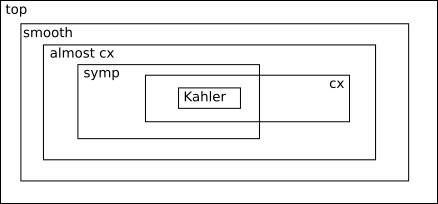
\includegraphics[width=0.8\linewidth]{mflds}
        \caption{Classes of manifolds.}%
        \label{fig:}
    \end{figure}
\end{thm}

\begin{proof}
    First, Freedman's $E_8$-manifold is not smoothable. Then $S^4$ has no almost complex structure. Third, $\P^2 \# \P^2 \# \P^2$ is not symplectic by Taubes and not complex by Kodaira-Siu. Fourth, $S^1 \times S^3$ admits a complex structure, but is not symplectic or K\"ahler. Fifth, the Kodaira-Thurston manifold is complex and symplectic, but not K\"ahler.
\end{proof}

\begin{rmk}
    Infinitely many examples in each subclass can be obtained by blowups $X \# \overline{\P}^2$.
\end{rmk}

\begin{exm}[Kodaira-Thurston Manifold]
    Let $G = \gen{\gamma_1, \gamma_2, \gamma_3, \gamma_4}$ act in $\R^4$ with coordinates $x_1, y_1, x_2, y_2$, where $\gamma_i$ increases the $i$th component by $1$ for $i = 1,3,4$, while $\gamma_2 = (x_1, y_1 + 1, x_2 + y_2, y_2)$. This is a free and properly dicontinuous action, so $X = \R^4 / G$ is a smooth manifold. Then $q: \R^4 \to X$ is the universal cover of $X$. Then we see that all $\gamma_i$ commute exept for $[\gamma_2, \gamma_3]$. Therefore $H_1 X = G/ [G,G]$, so $b_1 X = 3$. Therefore $X$ cannot be K\"ahler.
\end{exm}

\chapter{February 27}%
\label{cha:february_27}

\begin{exer}
    Let $f: X \to Y$ be a finite unbranched cover. Show that if $Y$ is symplectic, almost complex, complex, K\"ahler, projective, or Stein, then so is $X$.
\end{exer}

\section{Kodaira-Thurston Manifold}%
\label{sec:kodaira_thurston_manifold}

Recall the definition of the Kodaira-Thurston manifold $X$ as a quotient of $\R^4$ by a discrete group $G$ from last time.

\begin{rmk}
    We may obtain $X$ as a $T^2$-bundle over the torus.
\end{rmk}

To see this, note that we can project $X$ onto the first two coordinates. This is a map $f: X \to \R^2/\Z^2 = T^2$, where $\Z^2$ acts by shifts. To compute the fiber, note that $f^{-1}(0,0) = \R^2/\sim$, where $\sim$ identifies $(x_2, y_2) \sim (x_2 + 1, y_2)$ and $(x_2,y_2) \sim (x_2, y_2 + 1)$. Thus the fiber is a torus. The action of $\gamma_2$ becomes nontrivial monodromy.

To see the monodromy, note that if we move in the $x_1$-direction in the base, $\gamma_1$ identifies $(0,0,x_2,y_2)$ with $(1,0,x_2, y_2)$. However, in the $y_1$-direction, $\gamma_2$ identifies $(0,0,x_2, y_2)$ with $(0,1,x_2+y_2,y_2)$.

This gives us a description of the monodromy by the matrices $A = I_2, B = \begin{pmatrix}
    1 & 0 \\ 1 & 1
\end{pmatrix} \in SL_2(\Z)$.\footnote{$SL_2(\Z)$ is the mapping class group of the torus, which is the group of orientation preserving diffeomorphisms modulo isotopy.}

\begin{thm}[Thurston (1976)]
    The manifold $X$ is symplectic.
\end{thm}

\begin{proof}
    Choose the standard symplectic form $\omega_0 = dx_1 \wedge dy_1 + dx_2 \wedge dy_2$. Next we can see that $\gamma_i^*\omega_0 = \omega_0$ for all $i = 1, \ldots, 4$. The only one we need to check is $\gamma_2$, and we see that
    \[ \gamma_2^* \omega_0 = d x_1 \wedge d(y_1 + 1) + d(x_2 + y_2) \wedge dy_2 = dx_1 \wedge dy_1 + dx_2 \wedge dy_2 \]
    because $dy_2 \wedge dy_2 = 0$. Therefore each $\gamma_i$ is a symplectomorphism, so $G$ is a symplectomorphism of $(\R^4, \omega_0)$. Thus $\R^4 \to X$ is a covering with symplectic deck transformations. Thus there is an induced symplectic form $\omega$ on $X$.
\end{proof}

\begin{thm}[Kodaira (1969)]
    The Kodaira-Thurston manifold is complex.
\end{thm}

\begin{proof}
    Let $\alpha = dx_1, \beta = dy_1, \gamma = dx_2 - y_1 dy_2, \delta = dy_2$. Then this gives a $G$-invariant basis for $\Omega^1(\R^4)$. The only one we need to check is $\gamma$ with $\gamma_2$, and we see that
    \[ \gamma_2^* \gamma = d(x_2 + y_2) - (y_1 + 1)d (y_2 + 1) = dx_2 - y_1 dy_2. \]
    Then note that $\alpha, \beta, \delta$ are all closed, but $d \gamma = -dy_1 \wedge dy_2 = - \beta \wedge \delta = \delta \wedge \beta$.
    Then the dual basis
    \[ a = \frac{\partial}{\partial x_1}, b = \frac{\partial}{\partial y_1}, c = \frac{\partial}{\partial x_2}, d = -y_1 \frac{\partial}{\partial x_2} + \frac{\partial}{\partial y_2} \] 
    is a $G$-invariant basis for the Lie algebra of vector fields on $\R^4$. To see this, we only need to check $\gamma_2, d$, and we see
    \begin{align*}
        (\gamma_2)_* d &= -(y_1 + 1) \left( \frac{\partial x_1 }{\partial x_2} \frac{\partial}{\partial x_1} + \frac{\partial (y_1 + 1)}{\partial x_2} \frac{\partial}{\partial y_1} + \frac{\partial (x_2 + y_2)}{\partial x_2} \frac{\partial}{\partial x_2} + \frac{\partial y_2}{\partial x_2} \frac{\partial}{\partial y_2} \right) \\
                       &+ \left( \frac{\partial x_1 }{\partial y_2} \frac{\partial}{\partial x_1} + \frac{\partial (y_1 + 1)}{\partial x_y} \frac{\partial}{\partial y_1} + \frac{\partial (x_2 + y_2)}{\partial y_2} \frac{\partial}{\partial x_2} + \frac{\partial y_2}{\partial y_2} \frac{\partial}{\partial y_2} \right) \\
                       &= -(y_1 + 1) \frac{\partial}{\partial x_2} + \frac{\partial}{\partial x_2} + \frac{\partial}{\partial y_2},
    \end{align*}
    as desired. Now define $Ja = c, Jc = -a, Jb = d, Jd = -b$. Then we see that 
    \begin{align*}
        N_J(a,b) &= [Ja, Jb] - J[a,Jb] - J[Ja,b] - [a,b] \\
                 &= [c,d] - J[a,d] - J[c,b] - [a,b] \\
                 &= 0.
    \end{align*}
    Similarly, note that
    \begin{align*}
        N_J(b,d) &= [Jb, Jd] - J[b,Jd] - J[Db,d] - [b,d] \\
                 &= [d,-b] - J[b,-b] - J[d,d] - [b,d] \\
                 &= 0.
    \end{align*}
    Here we use the fact that all commutators vanish besides $[b,d] = -c$. Therefore $J$ is a complex structure on $\R^4$. In addition, the $G$-invariant basis for vector fields on $\R^4$ descends to a basis for vector fields on $X$. Also, $J$ descends to an integrable almost complex structure on $X$.
\end{proof}

\begin{cor}
    The Kodaira-Thurston manifold is complex and symplectic but not K\"ahler.
\end{cor}

\begin{rmk}
    The $G$-invariant basis $\alpha, \beta, \gamma, \delta$ descends to $\Omega^1(X)$. In addition, the symplectic form $\omega_0$ descends to the form
    \[ \omega = \overline{\alpha} \wedge \overline{\beta} + \overline{\gamma} \wedge \overline{\delta}. \]
\end{rmk}

\section{Algebraic Topology of $X$}%
\label{sec:algebraic_topology_of_x_}

For simplicity, we will drop the bars. Recall that $d \alpha = d \beta = d \delta = 0$, while $d \gamma = \delta \wedge \beta$. Also, note that $\alpha \wedge \alpha = \beta \wedge \beta = \delta \wedge \delta = 0$. Then recall that $\dim H^1(X, \R) = 3$ and note that $e(X) = 0$. Therefore, we obtain $b_2 = 4$.

We will write a basis for each cohomology and write the intersection form. We have
\[ H^1(X, \R) = \gen*{ [\alpha], [\beta], [\gamma] } \]
and
\[ H^2(X, \R) = \gen*{ [\alpha \wedge \beta], [\alpha \wedge \delta], [\gamma \wedge \beta], [\gamma \wedge \delta] }. \]
Next, we see that $H^3(X, \R) = \gen*{ [\beta \wedge \gamma \wedge \delta], [\alpha \wedge \gamma \wedge \delta], [\alpha \wedge \beta \wedge \gamma] }$ and $H^4(X, \R) = \gen*{[\alpha \wedge \beta \wedge \gamma \wedge \delta]}$.

Finally, we can see the intersection form is given by
\[ Q_X =  \begin{pmatrix}
    0 & 1 & 0 & 0 \\
    1 & 0 & 0 & 0 \\
    0 & 0 & 0 & -1 \\
    0 & 0 & -1 & 0
\end{pmatrix}. \]
From this, we see that $b^+X = B^-X = 2$, so $\sigma(X) = 0$.

\chapter{March 3}%
\label{cha:march_3}

\textbf{Note:} I was not here on this day. Notes were provided by Arthur Wang.

\section{Topology of Complex Manifolds}%
\label{sec:topology_of_complex_manifolds}

We will answer the following question:
\begin{quest}
    Are there any differential topological constraints for a symplectic $4$-manifold to admit a complex structure?
\end{quest}

Recall that all symplectic manifolds have an almost complex structure. Also, they have positive $b^+$.

\begin{thm}[Kodaira-Siu]
    If $X$ is a compact complex surface, $X$ is K\"ahler if and only if $b_1 X$ is even.
\end{thm}

We can consider $X$ with even first Betti number. Then if $X$ is complex, then it is K\"ahler. However, there are no constraints that come from Hodge theory. There are, however, more constraints from differential topology.

\begin{thm}[Hard Lefschetz]
    For $\omega$ the K\"ahler form, $L_{\omega}^k: H^{n-k}(M, \C) \to H^{n+k}(M, \C)$ is an isomorphism for all $k$. Here $L_{\omega}^k$ sends $\alpha$ to $\alpha \cup \omega^k$.
\end{thm}

This gives us Serre duality on Dolbeault cohomology.

\begin{rmk}
    All \textit{triple Massey products} on K\"ahler $M$ are zero: Let $a_1, a_2, a_3 \in H^*(M, \R)$ with $a_1 \cup a_2 = 0 = a_2 \cup a_3$. Then 
    \[ \gen{a_1, a_2, a_3} \in H^*(M, \R)/ a_1 \cup H^*M + H^*M \cup a_3 \]
    is defined as follows:

    Take $\alpha_i \in \Omega^*M$ with $a_i = [\alpha_i]$, so $\alpha_1 \wedge \alpha_2 = d \eta_{12}$ and $\alpha_2 \wedge \alpha_3 = d\eta_{23}$. Then
    \[ \gen{a_1, a_2, a_3} = [\eta_{12} \wedge \alpha_3 - (-1)^{\abs{a_1}} \alpha_1 \wedge \eta_{23}]. \]
\end{rmk}

There is a constraint from algebraic topology. Not all finitely presented groups are fundamental groups of K\"ahler manifolds. For example, if the abelianization of $\pi_1$ has odd rank, then $M$ is not K\"ahler. Also, $\pi_1$ that are nontrivial free products cannot be realized.

\begin{rmk}
    In dimension $4$, we can also use the Enriques-Kodaira classification of complex surfaces.
\end{rmk}

\section{Chern Classes}%
\label{sec:chern_classes}

We will define the canonical class of a complex or symplectic manifold. First, however, we need to define Chern classes. The $k$-th \textit{Chern class} of a complex vector bundle $E$ is a cohomology class $c_k(E) \in H^{2k}(M, \Z)$ and the total Chern class of $E$ is the sum $c(E) = c_0(E) + c_1(E) + \cdots$.

These uniquely satisfy the following axioms:
\begin{enumerate}
    \item $c_0(E) = 1$;
    \item (Naturality) For all $f:N \to M$, $c_k(f^*E) = f^*c_k(E)$.
    \item (Additivity) $c(E \oplus F) = c(E) \cup c(F)$.
    \item (Normalization) For the tautological line bundle over $\P^k$, we have $c = 1 - h$, where $h$ is the hyperplane class.
\end{enumerate}

\begin{rmk}
    The existence and uniqueness of the Chern classes follows from the theory of classifying spaces. Also, $c_k(E) = 0$ for all $k > \dim E$. The top Chern class is the Euler class, and for $E = TM$, $e(E)[M] = e(M)$, the Euler characteristic. Finally, Chern classes are invariant under isomorphism.
\end{rmk}

Note that if $M$ is symplectic, then the space of compatible $J$ is contractible and nonempty, so we can define Chern classes uniquely.

\begin{defn}
    The \textit{canonical class} of a (symplectic, complex) manifold $M$ is $K \coloneqq - c_1(M)$.\footnote{In algebraic geometry, this is defined as $\det T^*M$.}
\end{defn}

Now specialize again to the $4$-dimensional case. Then we have two cohomological invariants: The class of the symplectic form and the canonical class.

\begin{defn}
    We define $X$ to be minimal if $X$ is not a connected sum of another closed manifold and $\overline{\P}^2$.
\end{defn}

For minimal $X$, the we can define the \textit{symplectic Kodaira dimension} of $(X, \omega)$ as:
\[ \kappa(X) \coloneqq \begin{cases}
    - \infty & K \cdot [\omega] < 0 \text{ or } K^2 < 0 \\
    0 & K \cdot [\omega] = 0 \text{ and } K^2 = 0 \\
    1 & K \cdot [\omega] > 0 \text{ but } K^2 = 0 \\
    2 & K \cdot [\omega] > 0 \text{ and } K^2 > 0
\end{cases}. \]

For non-minimal manifolds, then we define the Kodaira dimension to be the Kodaira dimension of a minimal model.

\begin{rmk}
    There is a \textit{minimal madel program} for symplectic $4$-manifolds. One can always find a minimal symplectic $X$ such that $X' = X \# m \overline{\P}^2$.
\end{rmk}

\begin{rmk}
    By Taube's work on Seiberg-Witten invariants of symplectic manifolds, no other combinations for $K \cdot [\omega]$ and $K^2$ can occur.
\end{rmk}

This implies that $\kappa(X)$ is well-defined.

\begin{rmk}
    If $\kappa(X) = -\infty$, then $X$ is either rational or ruled.
\end{rmk}

\begin{rmk}
    When $X$ is K\"ahler, then its algebriac and symplectic Kodaira dimensions agree.
\end{rmk}

The general problem we want to solve is:
\begin{quest}
    For a given class of manifolds, what are the constraints on their algebraic topology? Which values can be realized as invariants of such manifolds?
\end{quest}


\chapter{March 5}%
\label{cha:march_5}

\section{Geography Problem}%
\label{sec:geography_problem_}

Today we will discuss problems of realizing certain algebraic invariants with a manifold admitting a certain structure. Let $X$ be a closed connected oriented smooth $4$-manifold. Which pairs of integers $(x,y) \in \Z^2$ can be realized as
\begin{enumerate}
    \item $(e(X), \sigma(X))$?
    \item $(c_1^2(X), c_2(X))$?
    \item $(c_1^2(X), \chi_h(X))$?
\end{enumerate}
Note that $c_1^2 = 2e + 3 \sigma$ and $\chi_h = \frac{e+\sigma}{4}$ (Noether's formula).
We will ask that $X$ is a minimal (irreducible smooth, almost complex, complex, symplectic, K\"ahler, projective) manifold. We will also fix $G = \pi_1 X$, which we will usually take to be trivial. We can also fix the type for $Q_X$.

\begin{rmk}
    Any pair determines the other pairs. Moreover, if $G = 1$, then by results of Serre, ..., Donaldson, then $e, \sigma, t$ determine $Q_X$. Then Freedman tells us that $Q_X$ determines the homeomorphism of $X$.
\end{rmk}

\section{Geography of Compact Complex Surfaces}%
\label{sec:geography_of_compact_complex_surfaces}

Let $X^4 = S$ be a minimal complex surface. Then we have the following:
\begin{description}
    \item[Kodaira] If $S$ is not Class VII,  rational, or ruled, then $c_1^2 \geq 0$ and $c_2 \geq 0$.
    \item[Noether] If $S$ is minimal and has Kodaira dimension $2$, then $c_1^2 \geq 2\chi_h - 6$.
    \item[Bogolomov-Minyaoka-Yau] If $S$ is not rational, ruled, or Class VII, then $c_1^2 \geq 9 \chi_h$.
    \item[Yau] If $c_1^2 = 9 \chi_h$, then $X$ is a complex ball quotient (if $X$ is not $\P^2$).
\end{description}

Moreover, we have a restricted \textit{complete} list for:
\begin{itemize}
    \item If $\kappa = -\infty$, then $X$ is rational or ruled.
    \item If $\kappa = 0$, then $X$ is Enriques, K3, $T^4$, or bielliptic.
    \item If $\kappa = 1$, then $X$ is elliptic.
\end{itemize}

\begin{thm}[Hirokawa, Xiao, Persson-Peters,...]
    All lattice points with $9 \chi_h \geq c_1^2 \geq 2 \chi_h - 2$ and $c_1^2 > 0$ are realized by minimal K\"ahler surfaces (mostly with $\pi_1$ trivial).
\end{thm}

\begin{exm}
    Note that $T^2$ and bielliptic surfaces lie at the origin. The ruled surfaces lie on $y = 8x$ in the third quadrant. $\P^2$ lies at the point $(1,9)$. The Class VII and Hopf surfaces lie on the negative $y$-axis. The elliptic surfaces lie on the positive $x$-axis, with the first two being Enriques and K3.
\end{exm}

\begin{thm}[Kodaira, Hirzebruch, Sommest, Persson, Moishezon-Teicher, Roulleau-Urzua]
    Several lattice points with $9 \chi_h > c_1^2 > 8 \chi_h$ can be realized arbitrary close to the BMY line with $\pi_1 = 1$.
\end{thm}

\begin{thm}[Mumford, Ishida-Cato, Keum, Prasad-Yeung, Cartwright-Steger]
    There are exactly $1 + 50 + 1$ surfaces the point $(1,9)$. These are fake $\P^2$ when $b_1 = 0$.
\end{thm}

\subsection{Geography of K\"ahler Surfaces}%
\label{sub:geography_of_k"ahler_surfaces}

We take the compact complex picture and simply remove the Class VII and Hopf surfaces.

\section{Geography of Simply-Connected Symplectic $4$-Manifolds}%
\label{sec:geography_of_simply_connected_symplectic_4_manifolds}

\begin{thm}[Taubes]
    If $X$ is not rational or ruled, then $c_1^2 \geq 0$.
\end{thm}

\begin{rmk}
    The Noether inequality fails in the symplectic case. This is due to Gompf, Fintushel-Stern, J. Park, who showed that all lattice points with $2 \chi_h - 6 > c_1^2 > 0$ are realized by minimal simply-connected symplectic $X$.
\end{rmk}

\begin{rmk}
    There are some restricted cases.
    \begin{itemize}
        \item If $\kappa = - \infty$, then $X$ is rational or ruled.
        \item If $\kappa = 0$, then the known examples are Enriques, K3, $T^4$, bielliptic, or $T^2$-bundles over $T^2$. We also know that any manifold with $\kappa = 0$ has the same rational homology as one of these (Li-Bauer).
        \item For $\kappa = 1$, Gompf and Fintuschel-Stern showed that there are infinitely more minimal symplectic $4$-manifolds than elliptic surfaces. In addition, by a result of Gompf, J. Park, Stipsicz, Akhmedov-Boldridge-Baykur-Kirk-Park, there are infinitely many sumplectic manifolds on almost all lattice points with $8 \chi_h \geq c_1^2 \geq 0$.
    \end{itemize}
\end{rmk}

\subsection{Five Fundamental Problems}%
\label{sub:five_fundamental_problems}

\begin{enumerate}
    \item Does every symplectic $4$-manifold which is not a ruled surface have $c_2 = e \geq 0$?
    \item (Symplectic BMY) Are there any symplectic $4$-manifolds that are not ruled that violate BMY?
    \item (Symplectic Yau) Are there any symplectic $4$-manifolds with $c_1^2 = 9c_2$ K\"ahler?
    \item (Symplectic Poincare Conjecture) Every symplectic $4$-manifold homeomorphic to $\P^2$ is diffeomorphic to it.
    \item (Symplectic Calabi-Yau Conjecture) Every symplectic $4$-manifold with $c_1 = 0$ is diffeomorphic to a K3 or a $T^2$-bundle over $T^2$.
\end{enumerate}

Solution to any of these problems will give us an A for the course regardless of what else happens during the semester. \.Inan\c{c} have us five problems so we wouldn't be fighting over them.

\chapter{March 10}%
\label{cha:march_10}

\textbf{Note:} I was away on this day; notes were provided by Arthur Wang.

\section{Darboux-Moser-Weinstein Local Theory}%
\label{sec:darboux_moser_weinstein_local_theory}

Let $\psi: M \times \R \to M$ be a smooth isotopy. This means that $\psi(-,t)$ is a diffeomorphism for all $t$ and $\psi(-,0)$ is the identity on $M$. From this flow we may obtain a time-dependent vector field $V_t$ such that
\[ V_t = \frac{d}{ds} \psi_s(\psi_t^{-1}(x)) \bigg\vert_{s = t}. \]
Equivalently, we have
\[ V_t \circ \psi_t = \frac{d}{dt} \psi_t \]
or
\[ (\psi_t)^* V_t = \frac{d}{dt} \psi_t.\]
From any time-dependent vector field $V_t$ we can find a $\psi_t$ solving the above ODE locally. If $V_t$ is compactly supported on $M$ (for example if $M$ is compact), then we can obtain $\psi_t$ globally.

\subsection{Moser's Method}%
\label{sub:moser_s_method}

We will construct an isotopy to match symplectic forms by constructing a time-dependent flow in an analogous fashion. Let $\omega_t \in \Omega^2M$ be a family of symplectic forms. Assume that 
\[ \frac{d}{dt} \omega_t = d \sigma_t \]
for some $\sigma_t \in \Omega^1 M$. We want to conclude that there exists an isotopy $\psi_t$ of $M$ such that 
\begin{equation}
    \psi_t^* \omega_t = \omega_0.
\end{equation}
This will imply that $(M, \omega_t)$ is symplectomorphic to $(M, \omega_0)$. If $M$ is compact, then it suffices to construct a flow satisfying (14.1).

Differentiating and integrating with respect to $t$, we see that (14.1) is equivalent to
\begin{align*}
    \frac{d}{dt} \psi_t^*\omega_t = 0 &\Leftrightarrow \psi_t^*\left(L_{V_t} \omega_t + \frac{d}{dt} \omega_t \right) \equiv 0 \\
                                      &\Leftrightarrow L_{V_t} \omega_t + \frac{d}{dt} \omega_t \equiv 0 \\
                                      &\Leftrightarrow i_{v_t} d \omega_t + d i_{v_t} \omega_t + d \sigma_t \equiv 0 \\
                                      &\Leftrightarrow d (i v_t \omega_t + \sigma_t) \equiv 0,
\end{align*}
by Cartan's magic formula, which means we must have
\[ i_{v_t} \omega_t + \sigma_t \equiv 0. \]
We need this equation to have a solution for all $t$, but it does because $\omega_t$ is nondegenerate. Therefore, we can take $V_t \coloneqq \mu_{\omega_t}^{-1}(- \sigma_t)$.

\begin{lem}[Moser's Isotopy]
    Let $M$ be a $2n$-dimensional manifold and $S \subset M$ be a compact submanifold. Let $\omega_0, \omega_1 \in \Omega^2 M$ be closed forms such that their restrictions to $T_S M$ are equal and nondegenerate on $S$. Then there exist open neighborhoods $N_i \supset S$ and a diffeomorphism $\psi: N_0 \to N_1$ such that $\psi^* \omega_1 = \omega_0$ and $\psi |_S = \mr{id}_S$.
\end{lem}
\begin{proof}
    Due to Moser's method, it suffices to show that there exists an open neighborhood $N_0 \supset S$ and $\sigma \in \Omega^1 N_0$ such that $\omega_1 - \omega_0 = d \sigma$ and $\sigma |_{T_SM} \equiv 0$.

    Using this, we can take $\omega_t = (1 - t) \omega_0 + t \omega_1$ on $N_0$. It is easy to see that $\omega_t$ is closed for all $t$. Then because nondegeneracy is an open condition, we can shrink $N_0$ to a smaller open neighborhood of $S$ to ensure nondegeneracy of $\omega_t$. Therefore we have a family of symplectic forms $\omega_t$ on $N_0$ such that $\omega_t = \omega_0 + t d \sigma$. Therefore we have a vector field $V_t$ whose flow is an isotopy $\psi_t$ of $N_0$, where we shrink $N_0$ further if needed so that $\psi_t^* \omega_t = \omega_0$. Because $\sigma$ is identically zero on $\sigma |_{T_SM}$, we have $V_t |_S \equiv 0$ and thus $\psi_t|_S = \mr{id}_S$.

    To show the existence of $N_0$, fix a Riemannian metric $g$ on $M$ and identify the normal bundle $\nu_S$ with $TS^{\perp}$. Consider the restriction of the exponential map $TS^{\perp} \to M$ around the open neighborhood of the zero-section:
    \[ U_{\ep} = \{ (s,u) \in TM \mid s \in S, v \in T_s S^{\perp}, \abs{v} < \ep \} \subset TS^{\perp}. \]
    Because $S$ is compact, $\mr{exp} |_{U_{\ep}}$ is a diffeomorphism for small enough $\ep$. Set $N_0 = \exp(U_{\ep})$. Define $\phi_t:N_0 \to N_0$ by $\phi_t(\exp(s,v)) = \exp(s, tv)$ so it is a diffeomorphism for $t > 0$ and $\phi_0(N_0) \subset S$. We also have $\phi_1 = \mr{id}_{N_0}$ and $\phi_t |_S = \mr{id}_S$.

    Therefore, for $\tau = \omega_1 - \omega_0^*$, we have $\phi_0^* \tau = 0$ and $\phi_1^* \tau = \tau$. Because $\phi_t$ is a diffeomorphism for $t > 0$, there exists a vector field
    \[ V_t \coloneqq \frac{d}{dt} \phi_t (\phi_t^{-1}) \]
    whose flow is $\phi_t$.
    Therefore, for $\delta > 0$, we have
    \begin{align*}
        \phi_1^* \tau - \phi_{\delta}^* \tau &= \int_{\delta}^1 \frac{d}{dt} \phi_t^* \tau \ dt \\
                                             &= \int_{\delta}^1 \phi_t^* \left( \mc{L}_{V_t} \tau + \frac{d}{dt} \tau \right)\ dt \\
                                             &= \int_{\delta}^1 \phi_t^* (i_{V_t} d \tau + d i_{v_t} \tau)\ dt \\
                                             &= \int_{\delta^1 d \phi_t^* (i_{V_t} \tau)}\ dt \\
                                             &= d \int_{\delta}^1 \phi_t^* (i_{V_t} \tau)\ dt \\
                                             &= d \sigma_{\delta}.
    \end{align*}
    Therefore, as $\delta \to 0^+$, $\sigma_{\delta \to \sigma}$, so $\omega_1 - \omega_0 = \tau = \phi_1^* \tau = \phi_1^* \tau - \phi_0^* \tau = d \sigma$. Thus $\omega_1 - \omega_0 = d \sigma$ and
    \[ \sigma |_{T_S M} = \int_0^1 \phi_t^* (i_{V_t} \tau)\ dt \bigg \vert_{T_S M} = \int_0^1 i_{V_t} \tau\ dt = \int_0^1 0\ dt = 0.\]
\end{proof}

    \begin{thm}[Darboux]
        Let $(M, \omega)$ be a symplectic manifold. Around any point $p \in M$, there exists a local coordinate chart $(U, \{x_i, y_i \})$ such that 
        \[ \omega = \sum_{i=1}^n dx_i \wedge dy_i. \]
        It follows that chart transitions for $M$ lie in $Sp(2n)$.
    \end{thm}

    \begin{proof}
        Using any symplectic basis for $T_p M, \omega|_p$, construct coordinates centered at $p$ and defined in some neighborhood $U'$ of $p$ such that $\omega = \sum dx_i' \wedge dy_i'$. Then apply Moser's lemma for $S = \{p\}, \omega_0 = \omega$, and $\omega_1 = dx_i \wedge dy_i$. Then there exist neighborhoods $U_0, U_1$ of $p$ and a diffeomorphism $\psi$ such that $\psi^* \omega_1 = \omega_0$ and $\psi(p) = p$. Then 
        \[ \omega |_{U_0} = \psi^* \left( \sum dx_i' \wedge dy_i' \right) = \sum d(x_i' \circ \psi) \wedge d(y_i' \circ \psi) = \sum dx_i \wedge dy_i. \]
    \end{proof}

    \chapter{March 12}%
    \label{cha:march_12}
    
    \textbf{Note:} I was away on this day; notes were provided by Arthur Wang.

    \begin{exer}
        Let $X$ be a closed, connected, oriented almost complex $4$-manifold.
        \begin{enumerate}
            \item Show that $X \# \overline{\P}^2$ is also almost complex;
            \item Show that any lattice point can be realized by a non-minimal simply-connected almost-complex manifold.
        \end{enumerate}
    \end{exer}

    \begin{exer}
        Let $\Sigma$ be a closed symplectic surface in a closed symplectic $4$-manifold $(X, \omega)$.
        \begin{enumerate}
            \item Show that any symplectic form on $\Sigma$ is determined up to isotopy by $\int_{\sigma} \omega$;
            \item Any symplectic neighborhood of $\Sigma$ is determined by $\Sigma \cdot \Sigma$ and $\int_{\Sigma} \omega$.
        \end{enumerate}
    \end{exer}

    We know there always exists a standard symplectic neighborhood of $S = \mr{pt}$. Generally, the goal is when $S \subset (M, \omega)$ is symplectic, Lagrangian, or (co)isotropic given some data on $\nu S$, the normal bundle of $S$. We will obtain a standard form for $\omega$ on a small tubular neighborhood of $S$.

    \section{$S$ is Symplectic}%
    \label{sub:_s_is_symplectic}
    
    Recall that there exists $J \in \mc{J}(M, \omega)$ such that $S$ is $J$-holomorphic. Then $\nu S = (TS)^{\omega} = (TS)^{\perp}$, so $\nu S$ is a symplectic vector bundle on $S$. Then recall that the isomorphism class is determined by the isomorphism class of the complex vector bundle $(\nu S, J)$. We will show that a neighborhood of $S$ is completely determined by $\omega |_S$ and the isomorphism class of $(\nu S, \omega)$.
    
    \begin{thm}[Weinstein, Symplectic neighborhood theorem]
        For $j = 0,1$, let $(M_j, \omega_j)$ be symplectic manifolds with compact symplectic submanifolds $S_j \subset M_j$ such that there exists a vector bundle isomorphism $\Phi: (\nu S_0, \omega_0) \to (\nu S_1, \omega_1)$ commuting with a symplectomorphism $\phi: S_0 \to S_1$. Then $\phi$ extends to a symplectomorphism $\psi$ of neighborhoods $N_i \supset S_i$ with $d \psi = \Phi$.
    \end{thm}

    \begin{proof}
        There exists $J_j \in \mc{J}(M_j, \omega_j)$ and compativle $g_j$ for which $S_j$ is $J_j$-holomorphic and $\nu S_j = TS_j^{\perp}$. Under these identifications, let $\varphi_j: \nu S_j \to M_j$ be the exponential maps. Then 
        \[\varphi = \varphi_1 \circ\varphi_0^{-1}\] 
        is a diffeomorphism from a neighborhood of $S_0$ to a neighborhood of $S_1$ where
        \[ \varphi^* \omega_1 |_{T_S M} = \omega_0 |_{T_S M}. \]
        Then use the Moser isotopy lemma for $S_0, \varphi^* \omega_1, \omega_0$.
    \end{proof}

    \section{$L$ is Lagrangian}%
    \label{sub:_l_is_lagrangian}

    In this case, $\dim L = n = \dim M / 2$, and we will see that the symplectomorphism class of a tubular neighborhood of $L$ is completely determined by the diffeomorphism class of $L$. Observe that if $L \subset (V, \omega)$ is a Lagrangian subspace of a symplectic vector space, then $\omega$ gives a canonical identification of $V/L$ with $L^*$.

    In the manifold case, if $L \subset (M, \omega)$ is Lagrangian, then $\nu L = T^* L$. Therefore a neighborhood of $L$ in $M$ is diffeomorphic to a neighborhood of the zero-section of the cotangent bundle $T^*L$.

    \begin{exm}[Canonical Symplectic Structure on the Cotangent Bundle]
        Let $L$ be any $n$-dimensional smooth manifold and $M = T^*L$. Then we will define the \textit{tautological $1$-form} $\lambda$ on $M$. We have the projection $\pi: M \to L$. For any $v \in M = T^* L$, $v$ is pulled back by $\pi$ to $\pi^* v \in T^*_v M$. Then we define $\lambda \in \Omega^1 M$ by
        \[ \lambda_v \coloneqq \pi^*(v) \in T^*_v M. \]
        The canonical symplectic structure $\omega$ on $M$ is $\omega = -d \lambda$, an exact form.

        In local coordinates, if $p_j$ are the coordinates on $L$ and $q_j$ are the cotangent coordinates, then we have
        \[ \lambda = \sum p_j d q_j. \]
        In fact $\lambda$ is characterized by the property that for all $\sigma \in \Omega^1 L$, $\sigma^* \lambda = \sigma$. By the local characterization, $\omega$ is symplectic. Finally, it is relatively easy to check that $L$ is Lagrangian in $T^*L$ (just use the local description).
    \end{exm}

    \begin{thm}[Weinstein, Lagrangian neighborhood theorem]
        Let $(M, \omega)$ be a symplectic manifold and $L \subset (M, \omega)$ be a compact Lagrangian submanifold. Then there exist neighborhoods $U$ of the zero section in $T^*L$ and $V$ of $L$ in $M$ and a diffeomorphism $\phi: U \to V$ such that $\phi^* \omega = - d \lambda$ that is the identity on $L$.
    \end{thm}

    \begin{exm}
        Let $L$ be a closed Lagrangian surface in a closed symplectic $4$-manifold $(X, \omega)$. Since $\nu L \simeq T^*L \simeq TL$ as bundles over $L$, then they have the same Euler class. Then we see that $e_{TL}[L] = e_{\nu L}[L]$, so $L \cdot L = e(L)$. Thus the isomorphism class of $\nu L$ is determined by the diffeomorphism type of $L$.

    By Theorem 15.5 there exists a Weinstein neighborhood $N(L) \subset (X, \omega)$ such that 
    \[N(L) \simeq \{ (q,p) \in T^* L \mid q \in L, \abs{p} < \ep \}. \]
    Observe that any radial push-off of $L$ in $N(L)$ is also Lagrangian.

    For $L = T^2$, note that $L \cdot L = e(L) = 0$ and $T^*L$ is trivial, so $N(L) \simeq T^2 \times B_{\ep}(0)$.
    \end{exm}

    \begin{exer}
        Let $X = \P^1 \times \P^1$ and $\omega = \pi_1^* \omega_{FS} + \pi_2^* \omega_{FS}$. Then recall that $\R\P^1$ is the fixed locus of complex conjugation on $\P^1$. Then $L = \R\P^1 \times \R\P^1$ is Lagrangian. How about a Lagrangian Klein bottle?
    \end{exer}

    \chapter{March 24}%
    \label{cha:march_24}
    
    \.Inan\c{c} decided on the following format for online class:
    \begin{itemize}
        \item He sends us lecture notes in a private Dropbox folder for us to read.
        \item There will be a Zoom discussion every Thursday at the usual time.
    \end{itemize}
    From now on, these notes will simply be a transcription of the notes we were sent.

    \section{Proof of Lagrangian Neighborhood Theorem}%
    \label{sec:proof_of_lagrangian_neighborhood_theorem}
    
     \begin{thm*}
        Let $(M, \omega)$ be a symplectic manifold and $L \subset (M, \omega)$ be a compact Lagrangian submanifold. Then there exist neighborhoods $U$ of the zero section in $T^*L$ and $V$ of $L$ in $M$ and a diffeomorphism $\phi: U \to V$ such that $\phi^* \omega = - d \lambda$ that is the identity on $L$.
    \end{thm*}

    \begin{proof}
        First note that if $(V, \omega)$ is a symplectic vector space with $L$ Lagrangian, then $JL$ is also Lagrangian for any almost complex structure $J$. Finally, $L \perp JL$ under a compatible metric $g$.

        For $(M, \omega)$ a symplectic manifold with $L \subset (M, \omega)$ Lagrangian and $J \in \mc{J}(M, \omega)$, the above applies to $J TL$. In addition, $JTL = TL^{\perp}$. Identifying this with $\nu L$, then we have an isomorphism with $T^* L$. Then for $g$ compatible with $\omega, J$, take the exponential map
        \[ \psi: T^*L \to M \] defined by
        \[ (q, v^*) \mapsto \exp(\beta(v^*)). \]
        Fixing the decomposition $T_{(q,0)} T^*L = T_qL \oplus T_q^*L$ for $q \in L$, write any $v \in T_{(q,0)} T^*L$ as $v = (v_0, v_1^*)$, then $d \omega_{(q,0)}(v) = v_0 + \beta(v_1^*)$. Therefore
        \begin{align*}
            \psi^* \omega_{(q,0)} (u,v) &= \omega_q(\psi_* u, \psi_*v) \\
                                        &= \omega_q(u_0 + \beta(u_1^*), v_0 + \beta(v_1^*)) \\
                                        &= \omega_q(u_0, v_0) + \omega_q(u_0, \beta(v_1^*)) + \omega_q(\beta(u_1^*), v_0) + \omega_q(\beta(u_1^*), \beta(v_1^*)) \\
                                        &= v_1^*(u_0) - u_1^*(v_0).
        \end{align*}

        On the other hand, at $q \in L$, $\left\{ \pdv{q_j} \right\}, \{ dq_j \}$ form a basis for $T_q L$ and $T_q^* L$, respectively. Therefore, for $u = \sum a_j \pdv{q_j} + \sum b_j dq_j$ and $v = \sum x_j \pdv{q_j} + \sum y_j dq_j$, then
        \begin{align*}
            d \lambda_{(q,0)}(u,v) &= \sum dp_j \wedge dq_j (u,v) \\
                                   &= \sum a_j x_j - y_j b_j \\
                                   &= \sum a_j x_j - \sum y_j b_j \\
                                   &= v_1^*(u_0) - u_1^*(v_0).
        \end{align*}
        Therefore $\psi^* \omega = -d\lambda$ on $T_{(1,0)} T^*L$ for all $q \in L$. The desired result then follows from Moser's isotopy lemma.
    \end{proof}

    \begin{exm}
        Let $L$ be a closed Lagrangian surface in a closed symplectic $4$-manifold $(X, \omega)$. Because $\nu L \cong T^*L \cong TL$ as bundles over $L$, then $e_{\nu L} [L] = e_{TL}[L]$, which implies that $L \cdot L = e(L) = 2 - 2g$.

        For $L \cong \Sigma_g$, then the diffeomorphism type of $L$ determines the isomorphism class of $\nu L$. By the Lagrangian neighborhood theorem, there exists a \textit{Weinstein neighborhood} $N(L) \subset (X, \omega)$ such that 
        \[ N(L) \cong \{ (q,p) \in T^* L \mid q \in L, \abs{p} < \ep \}. \]
        Ovserve that any ``radial push-off'' of $L$ in $N(L)$ is also Lagrangian. For $L = T^2$, then $L \cdot L = e(L) = 0$ and $T^*L = L \times \R^2$, so $N(L) = T^2 \times B_{\ep}(0)$.
    \end{exm}

    \chapter{March 26}%
    \label{cha:march_26}

    \section{More Local Theory}%
    \label{sec:more_local_theory}
    
    \begin{exm}
        Let $X = \P^1 \times \P^1 = S^2 \times S^2$ with $\omega = p_1^* (\omega_{FS}) + p_2^*(\omega_{FS})$. Then any $S^2 \times y_0$ or $x_0 \times S^2$ are symplectic submanifolds because it is easy to see that $i^* \omega = \omega_{FS}$.

        Now let $L = \R\P^1 \times \R\P^1$ which is the fixed locus of complex conjugation. Then $N(L) \cong T^2 \times \R^2$. Here, for $u,v \in T(S^1 \times S^1) \cong TS^1 \times TS^1$ with $u = (u_1, u_2)$ and $v = (v_1, v_2)$, then we have
        \begin{align*}
            i^* \omega(u,v) &= \omega_{FS}(d(p_1 \circ i)(-), d(p_1 \circ i)(-)) + \omega_{FS}(d(p_2 \circ i)(-), d(p_2 \circ i)(-)) \\
                            &= \omega_{FS}(u_1, v_1) + \omega_{FS}(u_2, v_2) \\
                            &= 0.
        \end{align*}
        Observe that for all $S_1 \to a \subset S^2$ and $S_1 \to b \subset S^2$, $a \times b$ is Lagrangian, so all $L_{a,b}$ are Lagrangian tori. All of these are boundaries, so they are topologically trivial.
    \end{exm}

    \begin{exer}
        Construct a Lagrangian Klein bottle in the same symplectic manifold. Also construct a homologically \textit{essential} Lagrangian torus in $\Sigma_g \times \Sigma_g$.
    \end{exer}

    \begin{rmk}
        There are similar theorems for isotropic manifolds (due to Weinstein) and coisotropic manifolds (due to Gotny) with more information on $\omega$ in a neighborhood.
    \end{rmk}

    \section{Another Application of Isotopy}%
    \label{sec:another_application_of_isotopy}

    Another application of Moser's isotopy conncerns equivalence of symplectic forms on a given manifold. Let $\omega_0, \omega_1$ be two symplectic forms on $M$. They they are 
    \begin{description}
        \item[Symplectomorphic] if there exists a diffeomorphism $\phi$ of $M$ such that $\phi^* \omega_1 = \omega_0$. 
        \item[Deformation equivalent] if there exists a smooth family $\omega_*$ of symplectic forms joining $\omega_0$ to $\omega_1$.
        \item[Isotopic] if there exists a deformation equivalence $\omega_*$ where $[\omega_*]$ is fixed.
        \item[Strongly isotopic] if there exists an isotopy $\phi_*$ of $M$ such that $\phi_1^* \omega_1 = \omega_0$.
    \end{description}
    Observe that strongly isotopic implies isotopic which implies deformation equivalent. Also strongly isotopic implies symplectomorphic. If $M$ is compact, then a result of Moser says that isotopic implies strongly isotopic.

    \begin{thm}[Moser Stability]
        Let $M$ be a closed symplectic manifold and $\omega_*$ be a smooth family of symplectic forms all in the same cohomology class. Then there exists an isotopy $\psi_*$ of $M$ such that $\psi_t \omega_t = \omega_0$.
    \end{thm}

    \begin{proof}[Sketch of Proof]
        To apply Moser's argument, we need a smooth family $\sigma_t \in \Omega^1 M$ such that $\frac{d}{dt} \omega_t = d \sigma_t$. Because the $\omega_t$ are in the same cohomology class, then $\tau_t = \dv{t} \omega_t$ must be exact. For each $t$, there exists $\sigma_t \in \Omega^1 M$ such that $\dd{\sigma_t} = \tau_t$. Such a \textit{smooth} family is constructed using the Poincare lemma and an inductive argument on the number of sets good covers of $M$.
    \end{proof}

    \begin{cor}
        Let $S_a = \qty{\omega \in \Omega^2 M \mid \omega \text{is symplectic and} [\omega] = a}$. Then for a closed symplectic manifold $M$, any two forms on the same path component of $S_a$ are symplectomorphic.
    \end{cor}

    \begin{exm}
        For $M = \Sigma$ with $\omega_0, \omega_1$ symplectic forms on $\Sigma$, then if $[\omega_0] = \omega_1$, there exists an isotopy $\psi_t$ of $\Sigma$ such that $\psi_1^* \omega_1 = \omega_0$.
    \end{exm}

    \chapter{March 31}%
    \label{cha:march_31}
    
    \section{Constructions of Symplectic Manifolds Through Surgery}%
    \label{sec:constructions_of_symplectic_manifolds_through_surgery}
    
    Here we will study important examples of \textit{symplectic} surgeries based on the local theory.

    \subsection{As Smooth Operations}%
    \label{sub:as_smooth_opera}

    \subsubsection{Blowup} 
    Here $M$ is replaced by 
    \[ M' = M \# \overline{\C\P}^n. \]

    \subsubsection{Blowdown}%
    \label{ssub:blowdown}
    
    Consider $\C\P^{n-1} \cong S \subset M$ with $\nu S \cong \mc{O}(-1)$. For $N(S) \cong \nu S$, we have $\partial N(S) \cong S^{2n-1}$. Then we replace $M$ with 
    \[ M' = (M \setminus N(S) \cup D^{2n}). \]

    \subsubsection{Fiber Connected Sum}
    Consider $S_i^{2n-2} \subset M_i^{2n}$ such that there exists an orientation \textit{reversing} bundle isomorphism $\overline{\phi}: \nu S_1 \to \nu S_2$. This induces $\psi: \partial N(S_1) \to \partial N(S_2)$. Then we replace $M$ with
    \[ M' = (M_1 \setminus N(S_1)) \cup_{\psi} (M_2 \setminus N(S_2)). \]
    
    \subsubsection{Torus Surgery}
    Let $L \subset X^4$ be a Lagrangian torus with trivial normal bundle. Then we replace $X$ by
    \[ X' = (X \setminus N(L)) \cup N(L) \]
    where $N(L)$ is twisted by the automorphism $\psi = \eta^{-1} \circ \phi \circ \eta$ for some diffeomorphism $\phi$ of $T^3$.
        
    \subsubsection{Rational Blowdown}
    Let $S_1, \ldots, S_{p-1}$ be embedded $S^2$ in $X^4$ such that the space $C_p$ formed by plumbing disc bundles in the following sequence:\footnote{This is taken from the original paper by Fintushel and Stern.}
    
    \centerline{\unitlength 1cm
    \begin{picture}(5,2)
    \put(.9,.7){$\bullet$}
    \put(1,.8){\line(1,0){1.3}}
    \put(2.2,.7){$\bullet$}
    \put(2.3,.8){\line(1,0){.75}}
    \put(3.3,.8){.}
    \put(3.5,.8){.}
    \put(3.7,.8){.}
    \put(4,.8){\line(1,0){.75}}
    \put(4.65,.7){$\bullet$}
    \put(.35,1.1){$-(p+2)$}
    \put(2.1,1.1){$-2$}
    \put(4.55,1.1){$-2$}
    \put(.45,.4){$u_{p-1}$}
    \put(2.1,.4){$u_{p-2}$}
    \put(4.55,.4){$u_1$}
    \end{picture}}
    embeds in $X^4$. Then $\partial C_p = \partial B_p = L(p^2, p-1)$. Here $B_p$ is a rational ball (meaning it has the same rational homology as the disc) with fundamental group $\Z/p\Z$. Then rational blowdown is the process of removing the interior of $C_p$ and replacing it with $B_p$. \textbf{Note taker:} I only understood this part after looking at the original paper by Fintushel and Stern.

    \subsection{As Symplectic Operations}%
    \label{sub:as_symplectic_operations}
    
    \subsubsection{Symplectic Blowup}%
    \label{ssub:symplectic_blowup}
    
    First recall the construction in the complex category. Here, the local model replaces $\C^n$ with the total space of $\mc{O}(-1)$, the tautological line bundle over $\P^{n-1}$.\footnote{For a more explicit presentation, see my algebraic geometry notes from Spring 2019.}

    Recall that there are two holomorphic projections $\pi: \widetilde{C}^n \to \C^n$ and $p: \widetilde{C}^n \to \P^{n-1}$, which correspond to the blowup map and the projection from $\mc{O}(-1)$. The fiber $E = \pi^{-1}(0)$ is called the \textit{exceptional divisor} of the blowup. The normal bundle of $E$ in $\widetilde{C}^n$ is simply $\mc{O}(-1)$, where $E$ is the zero section. Note that $c_1(L) = -H$, where $H$ is the hyperplane class. 

    On the other hand, the normal bundle $\nu \P^{n-1}$ of $\P^{n-1}$ in $\P^n$ is simply $\mc{O}(1)$. A complex line bundle on projective space is entirely determined by its first Chern class, so 
    \[ \overline{\nu E} \cong \nu \P^{n-1} \cong \P^n \setminus N(0), \]
    and therefore
    \[ \widetilde{\C}^n = (\C^n \setminus \{0\} ) \cup E = (\C^n \setminus N(0)) \cup \overline{\P^n \setminus N(0)} \cong \C^n \# \overline{\P}^n. \]

    \chapter{April 2}%
    \label{cha:april_2}

    \section{Complex Blowups}%
    \label{sec:complex_blowups}

    \textbf{Note taker:} A good reference for this lecture from the complex algebraic perspective is Griffiths and Harris, \textit{Principles of Algebraic Geometry.}

    \begin{exm}
        For $n = 2$, any exceptional divisor on a surface has self-intersection number $-1$. To see this, note that $c_1(L) = -h$.\footnote{For more details and a general form of this, see Griffiths and Harris.}
    \end{exm}

    It is possible to show that any local biholomorphic map $\C^n \to \C^n$ fixing the origin lifts to a local biholomorphic map on the blowup. Therefore, we can blow up any complex manifold $M$. From the topological point of view, this simply replaces $M$ with 
    \[ \widetilde{M} = M \# \overline{\P}^{n}. \] 
    In addition, it is easy to see that
    \[ c_1(\widetilde{M}) = c_1(M) - (n-1) E. \]
    In particular, for surfaces, we see that the canonical class of the blowup is
    \[ K_{\widetilde{X}} = \pi^* K_X + E. \]

    \begin{exm}
        Let $X = \Bl_1 \P^2$. Then we have a projection to $\P^1$ with fiber $\P^1$. In addition, the exceptional divisor is the zero section, so this is a \textit{Hirzebruch surface}. In addition, we have $F \cdot F = 0$ and $E \cdot F = 1$.
    \end{exm}

    \begin{exm}
        Let $C_0, C_1$ be two transverse, nonsingular cubics in $\P^2$. Then, we can consider the linear system generated by $C_0, C_1$ and resolve it. This will be a blowup of $\P^2$ in $9$ points. In addition, the linear system gives us a map to $\P^1$ which has generic fiber an elliptic curve. Thus $X \cong E(1)$, an \textit{elliptic surface}.
    \end{exm}

    \begin{exm}
        The local model for the blowups above can be seen in the standard example of ``resolution of singularities.'' Let $C = (z_1z_2 = 0) \subset \C^2$. Then the \textit{proper transform} of $C$ is simply a disjoint union of two lines.
    \end{exm}

    \begin{rmk}
        In general, one can blow up along any complex subvariety to resolve singularities.\footnote{However, the process for doing this is very complicated. The original proof of resolution of singularities by Hironaka is extremely long.}
    \end{rmk}
    
    \chapter{April 7}%
    \label{cha:april_7}
    
    \section{Symplectic Operations}%
    \label{sec:symplectic_operations}
    
    In a symplectic manifold, we can blow up following a local $J$-holomorphic model to obtain a new symplectic manifold $(M \# \overline{\P}^n, \widetilde{\omega})$, where $\widetilde{\omega}$ depends on some additional parameters.

    Let $\psi: B^{2n}(x) \to M$ be a symplectic embedding of a ball of radius $\lambda$. Then extend this by some $\ep >0$ and replace $\psi: B^{2n}(\sqrt{\lambda^2 + \ep^2})$ by the standard $\ep$-neighborhood of the zero section in $L$. Then recall that $L$ is the tautological bundle over $\P^{n-1}$, so we can write
    \[ \omega_{\lambda} = \pi^* \omega_0 + \lambda^2 pr^* \omega_{FS}. \]
    This is a K\"ahler form. Let $L(\ep)$ be the $\ep$-neighborhood of the zero section in $L$. Then
    \[ L(\ep) \setminus E \cong B^{2n}(\sqrt{\lambda^2 + \ep^2}) \setminus B(\ep), \]
    so we can glue symplectically. Moreover, we can normalize the construction so that:
    \begin{prop}[McDuff]
        The deformation class of $\wt{\omega}$ is unique, and the isotopy class is unique if we fix $\lambda$.
    \end{prop}
    
    \begin{thm}[McDuff, Symplectic Blowup]
        Given a symplectic manifold $(M, \omega)$, a compatible $J$, and a point $p_0 \in M$, we can symplectically blow up $M$ at $p_0$ and obtain a new symplectic manifold $(\wt{M}, \wt{\omega})$ such that $\pi: \wt{M} \to M$ is holomorphic, the exceptional divisor is $\wt{J}$-holomorphic, and 
        \[ [\wt{\omega}] = \pi^* [\omega] - \pi \cdot \lambda^2 [E]. \]
        Any two symplectic blowups of $(M, \omega)$ at points $p_0, p_1$ are equivalent up to symplectomorphism and deformation equivalence.
    \end{thm}

    \begin{rmks}
        \begin{enumerate}
            \item Complex blowup is infinitesimal, while symplectic blowup is local;
            \item Complex blowup is intrinsic, while symplectic blowup depends on $\lambda$.
            \item If $M$ is K\"ahler complex blowup is a symplectic blowup, but not the other way around.
            \item Blowup can simplify the topology of (singular) submanifolds and thei configurations, while complicating the topology of the ambient manifold. Also, blowing up decreases the symplectic volume.
            \item Complex curves in a complex surface intersect positively if if they are distinct. By a result of Gromov, the same holds for almost complex $J$.

                However, this is not true for symplectic surfaces in a symplectic $4$-manifold. For example, in the smooth category, we can move the exceptional divisor $E$ to $E'$, and then $E \cdot E' = -1$. Thus resolution of singularities does not behave well in the symplectic category.
        \end{enumerate}
    \end{rmks}

    \chapter{April 9}%
    \label{cha:april_9}
    
    \section{Symplectic Blowdown}%
    \label{sec:symplectic_blowdown}
    
    Suppose there exists a symplectic submanifold $\P^{n-1} \cong E \subset (M, \omega)$ and $\nu E \cong L$, then by the symplectic neighborhood theorem, there exists a small neighborhood $N(E)$ isomorphic to $L(\ep)$. Therefore, we can \textit{symplectically blow-down} $E$ to obtain a new symplectic manifold 
    \[ M' = (M \setminus N(E)) \cup B(\lambda). \]
    By a result of McDuff, only the choice of $E$ matters.

    \begin{thm}[McDuff, Symplectic Blowdown]
        Given a symplectic manifold $(M, \omega)$, compatible $J$, and symplectic exceptional divisor $E$, we can symplectcially blow down $M$ along $E$ and obtain a new symplectic manifold $(M', \omega')$ sith compatible $J'$ so that that the projection $M \to M'$ is holomorphic. Any two blowdowns along the same $E$ are symplectomorphic.
    \end{thm}

    \begin{exm}
        Let $X = \P^1 \times \P^1$ with the product K\"ahler structure. If we blowup at a point $p_0 = (x_0, y_0)$, then denote $F = x_0 \times \P^1$, $S = \P^1 \times y_1$ with $y_1 \neq y_0$. These are complex submanifolds of $X$. Then let $[\wt{F}], [\wt{S}]$ be the proper transforms of $F, S$ in the blowup, we see that $[\wt{F}] = \pi^* [F] - E, [\wt{S}] = \pi^*[S] - E$.\footnote{\textbf{Note Taker:} This can be computed easily using standard techniques in algebraic geometry.}

        Now we blow down $\wt{F}$ and obtain $(S', \omega')$. Then note that $S$ is another symplectic exceptional sphere, which can be blown down again to obtain $\P^2$. Therefore $\wt{X}$ has two different minimal models.

        If we perform only complex blowdowns, then $X'' = \P^2$ because there exists a unique symply-connected complex surface on the BMW line. Thus $X' = \Bl \P^2$. If we perform symplectic blowdowns without worrying about complex structures, then $E \to E''$, and there exists a symplectic $E'' \cong \P^1$ with self-intersection $+1$.
    \end{exm}

    \begin{rmk}
        Note that the local model of the blowup is always the same, so we must always have $[\wt{F}]^2 = F^2 - 1$.
    \end{rmk}

    \begin{prop}[McDuff]
        If there exists a homologically essential degree of non-negative self-intersection in $(X, \omega)$, then $X$ is rational or ruled.
    \end{prop}

    \begin{rmk}
        This implies that $(X'', \omega'') \cong (\P^2, \omega_{FS})$ in our example.
    \end{rmk}

    \chapter{April 14}%
    \label{cha:april_14}
    
    \section{Symplectic Fiber Connected Sum}%
    \label{sec:symplectic_fiber_connected_sum}
    
    Let $(M_i, \omega_i)$ be symplectic manifolds of dimension $2n$ and let $S_i$ be codimension $2$ symplectic submanifolds. Here $\nu S_i$ is determined by the Euler number of $S_i$. Then there exists an orientation-reversing bundle isomorphism $\nu S_1 \to \nu S_2$ if there is an orientation preserving isomorphism $S_1 \to S_2$ and $e_1 = - e_2$. 

    For the symplectic construction, we want the orientation-reversing bundle isomorphism to be a symplectomorphism. For simplicity, let's suppose the normal bundle is trivial. 

    Then by the symplectic neighborhood theorem, there exists a neighborhood $N(S_i)$ such that $N(S_i) \cong B^2(r_0) \times S_i$. For any $0 < r_1 < r_0$, we have a symplectic submanifold, the annulus $A^2(r_1,r_0) \subset B^2(r_0)$. Then given a symplectomorphism between the bundles, we obtain a symplectomorphism $A^2(r_1, r_0) \times S_1 \to A^2(r_1,r_0) \times S_2$ by switching the two boundary components of the annulus. This gives us a symplectomorphism
    \[ \overline{\psi} N(S_1) \setminus \xi^{-1}(B^2(r_1) \times S_1) \to N(S_2) \setminus \xi)2^{-1}(B^2(r_0) \times S_2), \]
    where $\xi_i$ is the isomorphism $N(S_i) \to B^2(r_0) \times S_i$. Therefore, we can set
    \[ M = (M_1 \setminus N_1(S_1)) \cup_{\overline{\psi}} (M_2 \setminus N_2(S_2)). \]

    \begin{rmks}
        \begin{enumerate}
            \item The same construction extends to the case $0 \neq e_1 = -e_2$, where instead of the product, we take an annular fiber bundle isomorphism. 
            \item $M$ is determined up to orientation preserving diffeomorphism by the pairs $(M_i, S_i)$, trivializations $\xi_i$, and the symplectomorphism $\phi: S_1 \to S_2$. Often the trivializations are understood from the context, for example when the $S_i$ are fibers of a fibration.
            \item When $2n = 4$, there exists a symplectomorphism $\phi: S_1 \to S_2$ if they are diffeomorphic and have the same volume. The latter can always be achieved by multiplying one of the $\omega_i$ by a constant. Thus it is enough to have $g(S_1) = g(S_2)$ and $S_1^2 = -S_2^2$. 
            \item When $2n = 2$, then the $S_i$ are each a single point, and the fiber connected sum is the same as the regular connected sum.
            \item Note that one cannot find a symplectomorphism of $B^{2n}(r_0) \setminus B^{2n}(r_1)$ when $n > 0$. Otherwise, we could glue two symplectic discs to form a symplectic sphere.
        \end{enumerate}
    \end{rmks}

    \begin{thm}[Symplectic Fiber Connected Sum]
        For $j = 1,2$ let $(M_j, \omega_j)$ be $2n$-dimensional symplectic manifolds with $(2n-2)$-dimensional submanifolds $S_j$. If there exists a symplectomorphism $\phi: S_i \to S_2$ and the Euler numbers $e_j$ of $\nu S_j$ satisfy $e_1 = -e_2$, then there exists a new symplectic manifold $(M, \omega) = (M_1 \omega_1) \#_{\phi} (M_2, \omega_2)$.

        For $2n = 4$, it is enough to have $g(S_1) = g(S_2)$ and $S_1^2 = -S_2^2$.
    \end{thm}

    \begin{thm}[Usher]
        If the $X_j$ are minimal and $g(S_j) \geq 1$, then $X = X_1 \#_{S_1 = S_2} X_2$ is minimal.
    \end{thm}

    \chapter{April 16}%
    \label{cha:april_16}
    
    \begin{exm}
        Consider $E(1) = \Bl_9 \P^1$ and $F$ a smooth fiber. Then we know $F^2 = 0$. If we let $(E(2), \omega_2) = (E(1), \omega_1) \# (E(1), \omega_1)$, and more generally, 
        \[ (E(n), \omega_n) = (E(n-1), \omega_{n-1}) \# (E(1), \omega_1), \]
        then the elliptic fibration on $E(1)$ extends to $E(n)$. In fact, all $E(n)$ are K\"ahler. In fact, the pullback of $E(1)$ along $z \mapsto z^n$ is birational to $E(n)$.
    \end{exm}

    Now we will study the algebraic topology of $X = E(2)$. We know that 
    \[ \pi_1(X) \cong \pi_1(E(1) \setminus N(F)) * \pi_1(E(1) \setminus N(F)) \]
    Here, $\pi_1(E(1)) \cong \pi_1(E(1) \setminus N(F)) * \pi_1(N(F)) \cong \pi_1(E(1) \setminus N(F)) * \Z^2$. Recall that $F$ is a $9$ times blown-up smooth cubic, so $\pi_1(E(1)) \cong \pi_1(E(1) \setminus N(F)) = F$, and thus $\pi_1(X) = 1$. Next, we know that 
    \[ e(X) = 2e(E(1) \setminus N(F)), \] 
    and $e(E(1)) = e(E(1) \setminus N(F))$, so $e(E(2)) = 24$. In addition, we can show that
    \[ \sigma(E(2)) = 2 \sigma(E(1)) = -16. \]
    In general, $E(n)$ is simply connected, $e(E(n)) = 12n$, and $\sigma(E(n)) = -8n$. Then, we see that $K^2 = 2e + 3 \sigma = 0$. Therefore, all $E(n)$ have Kodaira dimension.

    \begin{prop}[Adjunction Formula]
        If $\Sigma \subset (X, \omega)$ is a symplectic surface, then $-e(\Sigma) = [\Sigma]^2 + K_X \cdot \Sigma$. In particular, it holds for any $J$-holomorphic $\Sigma$.
    \end{prop}

    \begin{proof}
        Note that $TX|_{\Sigma}$ is a symplectic vector bundle. In particular, $T \Sigma$ is a symplectic subbundle. Therefore, we can write
        \[ T_{\Sigma} X = T \Sigma \oplus T \Sigma^{\omega} = T \Sigma \oplus \nu \Sigma, \]
        so we have
        \[ c_1(X) = c_1(T \Sigma) + c_1(\nu \Sigma). \]
        Applying this to intersection with $\Sigma$ gives us the desired formula.
    \end{proof}

    From this, we see that any section of $E(2)$ has self-intersection $-2$. In general, there exists a symplectic sphere of self-intersection $-n$ in $E(n)$. Therefore $K \cdot S = n-2$, so $K$ is not torsion for $n \neq 2$. Thus $E(n)$ has Kodaira dimension $1$ for $n \geq 3$, while $E(2)$ is a K3 surface.

    \chapter{April 21}%
    \label{cha:april_21}
    
    \section{Luttinger Surgery}%
    \label{sec:luttinger_surgery}
    
    This is a symplectic surgery along a Lagrangian torus. When $2n = 4$, $L$ is an embedded Lagrangian torus inside a symplectic $4$-manifold $(X, \omega)$. Let $\gamma$ be a loop inside $L$ which is co-oriented.

    Here $N(L) \cong \nu L \cong T^*L \cong T^2 \times \R^2$ is the trivial bundle. Therefore we can perform a torus surgery along $L$ in $X$. To construct an explicit model, note that by Weinstein, there exists a neighborhood $N(L)$ of $L$ diffeomorphic to $T^*L$, where $L$ corresponds to the zero-section. Moreover, $T^*L \cong T^2 \times \R^2$, where we can identify $T^2 = \R^2/\Z^2 = q(\R^2)$ with coordinates $x_1, x_2$ and $\gamma = \R/\Z = q(\R)$ with co-orientation $\pdv{x_2}$.

    Thus for $(y_1, y_2)$ the dual coordinates in the cotangent fibers, we have
    \[ \xi: (N(L), \omega) \xrightarrow{\cong} (T^2 \times \R^2, dx_1
    \wedge dy_1 + dx_2 \wedge dy_2) \] where $L \longleftrightarrow T^2
    \times 0$. In fact, any $T^2 \times \mr{pt}$ is Lagrangian. We call
    $\xi$ a \textit{Lagrangian framing}.

    Let $r > 0$ such that $U_r = \R^2 \times \Z^2 \times [-r,r]^2 \subset \xi(N(L))$. Then let $\mc{X}: [-r,r] \to [0,1)$ be a $C^{\infty}$ step function such that $\mc{X}(t) = 0$ for all $t \leq -\frac{r}{2}$ and $\mc{X}(t) = 1$ for $t \geq \frac{r}{3}$ and $\mc{X}'(t) > 0$ in between. Finally, we want
    \[ \int_{-r}^r t \mc{X}'(t) \dd{t} = 0. \]
    For any $k \in \Z$, define $\phi_i: (U_r \setminus U_{r/2}) \to (U_r \setminus U_{r/2})$ by
    \[ \phi_k(x_1,x_2,y_1,y_2) = \begin{cases}
        (x_1 + k \mc{X}(y_1), x_2, y_1, y_2) & y_2 \geq \frac{r}{2} \\
        (x_1,x_2,y_1,y_2) & \text{otherwise}
    \end{cases}. \]
    We can check that $\phi_k$ is a symplectomorphism.

    Luttinger surgery replaces $(X, \omega)$ with $(X',\omega')$, where
    \[ X' = (X \setminus \xi^{-1}(U_{r/2})) \cup U_r \]
    and $\omega' = \omega$ on $X$ and $\omega_0$ on $U_r$. We will denote $X' = X(L, \gamma, k)$. Note that $(L, \gamma, k)$ determine $X$ up to orientation-preserving diffeomorphism:
    \begin{itemize}
        \item $L$ and the Lagrangian framing $\xi$ determine $N(L)$;
        \item The co-oriented $\gamma$ determines the $x_1$ direction and the choice of $k$ determines $\phi_k$;
        \item Different $\mc{X}$ determine isotopic $\phi_k$.
    \end{itemize}

    Under the Lagrangian framing, $\gamma$ can be pushed off to a curve $\gamma'$ in a neighborhood of $L$. The image of $\gamma'$ under regluing determines the diffeomorphism typd of $X'$ by handle theory.

    \begin{thm}[Luttinger, Auroux-Donaldson-Katzarkov]
        $(X',\omega') = (X(L, \gamma, k), \omega')$ is uniquely determined up to symplectomorphism.
    \end{thm}

    \begin{exm}
        Let $\omega_{\Sigma}$ be a symplectic form on $\Sigma$ and $\phi$ be a symplectomorphism of $(\Sigma, \omega_{\Sigma})$.
        \[ Y_{\phi} \coloneqq [0,1] \times \Sigma / (1,x) \cong (0,\phi(x)) \]
        and 
        \[ X \coloneqq (\R \times \R \times \Sigma) / G \cong S^1 \times Y_{\phi}, \]
        where $G$ is generated by $g_1(s,t,x) = (s+1,t,x)$ and $g_2(s,t,x) = (s,t+1,\phi(x))$. Because both of these are symplectomorphisms, $X$ is a symplectic manifold. Observe that $X$ is a $\Sigma$-bundle over $T^2$ with has monodromy the identity in the $s$-direction and $\phi$ in the $t$-direction. 

        Now let $\gamma$ be a loop in a fiber $F \cong \Sigma_g$ of this bundle. Then $L \coloneqq S^1 \times T_0 \times \gamma$ is a Lagrangian torus inside $(X, \omega)$. Therefore, we have an isomorphism
        \[ X(L, \gamma, k) = S^1 \times Y_{T_{\gamma_0}^k \circ \phi}, \]
        where $T_{\gamma_0}$ is a positive Dehn twist along $\gamma$ for the opposite co-orientation. This gives a new $\Sigma$-bundle over $\T^2$ with trivial monodromy $s$ in the $s$-direction and monodromy $T_{\gamma_0}^k \circ \phi$ in the $t$-direction.

        In particular, for $X = T^4$ and $\gamma = (s_0,t_0) \times S^1 \times \mr{pt}$, we get $X(L, \gamma, 1)$ is the Kodaira-Thurston manifold.
    \end{exm}

    \begin{rmk}
        By a result of Ho-Li, there exists an embedded surface $S \subset X \setminus N_1(L) = X_0$ such that for $\iota_X: X_0 \to X$, $(\iota_X)_* [S] = K_{\omega}$ and for $\iota_{X'}: X_0 \to X'$, $(\iota_{X'})_* [S] = K_{\omega'}$.\footnote{I am being deliberately sloppy with homology and cohomology here. Use Poincar\'e duality to correct the RHS of both equations.}

        When $X, X'$ are minimal, we can compute the Kodaira dimensions:
        \begin{align*}
            K^2_{\omega} = \int_S K_{\omega} = \int_{S'} K_{\omega'} = K_{\omega'}^2; \\
            K_{\omega} \cdot [\omega] = \int_S \omega = \int_S' \omega' = K_{\omega'} \cdot [\omega']. 
        \end{align*}
        Therefore, the Kodaira dimensions are the \textit{same!}.
    \end{rmk}

    \begin{thm}[Enriques-Kodaira]
        There exist finitely many K\"ahler manifolds $C \supset T^4$ with Kodaira dimension $0$.
    \end{thm}

    Now, any $\Sigma_g$-bundle over $\Sigma_n$ with $g,h \geq 1$ is \textit{acyclic} ($\pi_2 = 0$). Therefore, it is minimal. Then for all $k \in \Z$, if we set $X_k \coloneqq T^4(L, \gamma, k)$ as above, then every $T^2$ bundle over $T^2$ is a minimal symplectic manifold with the same Kodaira dimension as $T^4$. We can show that $H_1(X_k) = \Z^3 \oplus \Z/k\Z$, so we get only symplectic manifolds, not K\"ahler manifolds.

    \chapter{April 23 and 28}%
    \label{cha:april_23_and_28}
    
    Note that \.Inan\c{c} posted both of these lectures in the same file.

    \section{Fundamental Groups of Symplectic Manifolds}%
    \label{sec:topology_of_symplectic_4_manifolds}
    
    \begin{thm}[Gompf]
        Any finitely presentable group $G$ is the fundamental group of a closed symplectic $4$-manifold.
    \end{thm}

    \begin{rmk}
        The analogous result is true in any larger dimension by taking products with $\C\P^1$.
    \end{rmk}

    Our proof of Theorem 25.1 will use the following trick due to Gompf of turning homologically essential Lagrangian submanifolds into symplectic submanifolds in dimension $4$.

    \begin{prop}
        Let $(X^4, \omega)$ be a closed symplectic $4$-manifold and $F_1, \ldots, F_r$ be closed, connected, oriented, disjoint embedded Lagrangian submanifolds of $(X, \omega)$. Suppose that $[F_1], \ldots, [F_r] \in H_2(X, \R)$ lie in an affine subspace that does not contain $0$. Then there exists an arbitrarily small perturbation $\omega'$ of $\omega$ such that $(X, \omega')$ is symplectic and the $F_i$ are symplectic submanifolds (respecting the given orientations and of equal area).
    \end{prop}

    \begin{proof}
        The affine subspace hypothesis implies there exists a linear function on $H_2(X, \R)$ evaluating to $1$ on each $[F_i]$. Therefore, there exists a closed $2$-form $\eta$ such that
        \[ \int_{F_i} \eta = 1 \] for all $i$. Then let $\omega_i$ be a symplectic form on $F_i$ with $\int_{F_i} \omega_i = 1$. Thus for $j_i: F_i \to X$ the inclusion map, we have
        \[ \int_{F_i} \omega_i - j_i^* \eta = 0, \]
        so $\omega_i - j^* \eta = d \alpha_i$ for some $1$-form $\alpha_i$ on $F_i$. Now extend $\alpha_i$ to a form on $X$ by first pulling it back over a small tubular neighborhood $N(F_i)$. Then we smoothly taper it to zero outside of $N(F_i)$. Therefore
        \[ \eta' \coloneqq \eta + \sum_{i=1}^r d \alpha_i \]
        is a closed $2$-form such that $j_i^* \eta' = \omega_i$ for all $i$. If we set $\omega' = \omega + t \eta'$ for a fixed $t > 0$, $\omega'$ is closed. Because nondegeneracy is an open condition, $\omega'$ is also nondegenerate for small enough $t$. Moreover, $j_i^* \omega' = 0 + t \omega_i$ is a symplectic form on $F_i$ with area equal to $t$ for all $i$.
    \end{proof}

    \begin{rmk}
        Now suppose $\omega' = \omega + t \eta$ is degenerate at $x \in X$ for some $t > 0$. Then there exists some $0 \neq u \in T_x X$ such that $\omega(u,v) + t \eta(u,v) = 0$ for all $v \in T_x X$. If this is also true for $t/2$, then $\omega(u,v) = 0$ for all $v \in T_x X$. Thus for each $x \in X$, there exists $t_x > 0$ for which $\omega'$ is nondegenerate. Because $X$ is compact, we can find a global $t$.
    \end{rmk}

    \begin{proof}[Proof of Theorem 25.1]
        Fix a finite presentation $\ip{g_1, \ldots, g_k}{r_1, \ldots, r_{\ell}} \cong G$. Then let $F = \Sigma_k$ and let $a_1, b_1, \ldots, a_k, b_k$ be a standard collection of oriented embedded circles on $F$. Here, $a_i \cdot b_j = \delta_{ij}$.When suitably attached to a base point, $a_1, b_1, \ldots, a_k, b_k$ are generators of $\pi_1 F$. Here,
        \[ \pi_1 F \cong \ip{a_1,b_1,\ldots, a_k, b_k}{[a_1,b_1]=\cdots=[a_k,b_k]=1}. \]
        Therefore, $\pi_1 F / N(b_1, \ldots, b_k) \cong \ev{a_1, \ldots, a_k}$, the free group in the $a_i$. Under the above isomorphism, each condition $r_i$ is a word in $a_i^{\pm 1}$. 

        Let $\gamma_i$ be a smooth, immersed, oriented circle in $F$ with only double points representing this word. We can then add handles at self-intersection points of each $\gamma_i$, so each $\gamma_i$ is embedded in some $\Sigma_k \# M T^2$. We also add handles so each $\gamma_i$ is \textit{non-separating}.

        Let $F = \Sigma_g$, where $g = k + M$ be this bigger surface, where we have additional $a_i,b_i$ for $i = k+1, \ldots, g$. For $S = \qty{b_1, \ldots, b_k, \gamma_1, \ldots, \gamma_k, a_{k+1}, b_{k+1}, \ldots, a_g, b_g}$, we have $\pi_1 F / N(S) \cong G$. 

        For $F \cong \Sigma_g$ and $S$ a collection of circles as above, we can assume $g \geq 1$ by adding trivial relations if needed. To simplify the notation, label the circles in $S$ as $c_i$ for $i = 1, \ldots, m$.

        Take $X = T^2 \times F$ with the product symplectic form. For $S^1 = [0,1]/0 \sim 1$, let $0 < t_1 < \cdots < t_m < 1$. Then the embedded tori $L_i \coloneqq S^1 \times t_i \times c_i$ are all Lagrangian in $(X, \omega)$. Moreover, since each $c_i$ is non-separating in $G$, there exists $d_i \subset F$ such that $\abs{c_i \cap d_i} = 1$. Therefore, the torus $D_i \coloneqq \mr{pt} \times S^1 \times d_i$ is dual to $L_i$.

        Applying Proposition 25.3 repeatedly, we can perturb $\omega$ to $\omega'$ so that all $L_i$ are now symplectic. Clearly $L_i^2 = 0$, so each is a symplectic torus with trivial neighborhood.

        Therefore, $\pi_1 X \cong \pi_1 T^2 \oplus \pi_1 F$. Let $p_0 \in F \setminus S$. Then $L_0 = T^2 \times p_0$ is also a symplectic torus with trivial neighborhood and disjoint from the $L_i$.

        Let $(X_G, \omega_G)$ be the symplectic manifold we obtain by symplectic fiber sum along $L_0, \ldots, L_m$ with $m+1$ copies of $E(1)$ along a smooth fiber $F$. Because $\pi_1(E(1) \setminus F) = 1$, we apply Seifert-van Kampen to obtain
        \[ \pi_1(X_G) = \pi_1(X) / N(\mathbf{x}, \mathbf{y}, c_1, \ldots, c_m) \cong G. \qedhere \]
    \end{proof}

    \begin{rmks}
        \begin{enumerate}
            \item We can get infinitely many many symplectic manifolds with the same fundamental group $G$ by connected sum with $E(n)$ instead of $E(1)$.
            \item By a result of Usher, $X_G$ is minimal.
            \item $\kappa (X_G) = 1$.
            \item There are infinitely many non-K\"ahler symplectic manifolds, all on the ``$x$''-line,
        \end{enumerate}
    \end{rmks}

    \begin{exm}
        For example, there exists a closed symplectic $4$-manifold $X$ with $\pi_1 X = \Z * \Z$.
    \end{exm}
    


    
    
    
\end{document}
